\chapter{著名定理的证明}

\section{海伦公式}
三角形三边长分别为 $ a,b,c $,令 $ s=\dfrac{a+b+c}{2} $,则三角形面积为 $ \sqrt{s(s-a)(s-b)(s-c)} $。
\begin{figure*}[htbp]
\centering
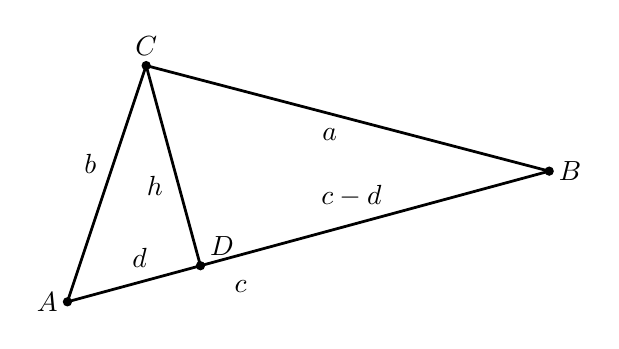
\begin{tikzpicture}[]
\coordinate[label=left:$A$] (A) at (-3,0);
\coordinate[label=right:$B$] (B) at (3.1184,1.6593364341085264);
\coordinate[label=above:$C$] (C) at (-2,3);
\coordinate[label=above right:$D$] (D) at (-1.310642335049465,0.4581610753943723);
\draw [line width=1pt] (A) to[edge label=$b$] (C);
\draw [line width=1pt] (B) to[edge label=$a$] (C);
\draw [line width=1pt] (B) -- (A);
\draw [line width=1pt] (D) to[edge label=$h$] (C);
\draw (-2.3,0.8) node[anchor=north west] {$d$};
\draw (-1,0.4) node[anchor=north west] {$c$};
\draw (0.1,1.6) node[anchor=north west] {$c-d$};
\tkzMarkRightAngle[line width=1pt](A,D,C)
\foreach \p in {A,B,C,D}
	\fill[fill=black,draw=black,thick] (\p) circle (1.25pt);
\end{tikzpicture}
\end{figure*}
\begin{proof}
如上图,由勾股定理:
\begin{align*}
b^2&=h^2+d^2 \\
a^2&=h^2+(c-d)^2
\end{align*}

上面两个式子相减:
\begin{align*}
a^2-b^2&=c^2-2cd \\
d&=\frac{b^2+c^2-a^2}{2c}
\end{align*}

代入第一个式子:
\begin{align*}
h^2&=b^2-d^2=(b+d)(b-d) \\
&=(b+\frac{b^2+c^2-a^2}{2c})(b-\frac{b^2+c^2-a^2}{2c}) \\
&=\frac{(2bc+b^2+c^2-a^2 )(2bc-b^2-c^2+a^2 )}{4c^2} \\
&=\frac{((b+c)^2-a^2 )(a^2-(b-c)^2 )}{4c^2} \\
&=\frac{(b+c+a)(b+c-a)(a+b-c)(c+a-b)}{4c^2} \\
&=\frac{2s\cdot 2(s-a)\cdot 2(s-c)\cdot 2(s-b)}{4c^2} \\
&=\frac{4s(s-a)(s-b)(s-c)}{c^2} 
\end{align*}

求面积:
\begin{equation*}
Area=\frac{1}{2} hc=\sqrt{\frac{1}{4} h^2 c^2 }=\sqrt{s(s-a)(s-b)(s-c)}
\end{equation*}

\end{proof}

\newpage
%------------------------------------------------------------------------------%
\section{悬链线方程}
质量均匀的绳子自由悬挂,只考虑自身重量,求形成的曲线形状。


\begin{figure*}[htbp]
\centering
\begin{tikzpicture}[scale=1.5,domain=0:5]
\coordinate (O) at (0,0);
\coordinate[label=above left:$T_0$] (A) at (-1.5,0);
\coordinate (B) at (3.2117777777777774,1.5914986998664422);
\coordinate (C) at (3.4855555555555555,1.944112448982997);
\coordinate (D) at (3.73,2.305416047938065);
\coordinate (E) at (4.67,1.944112448982997);
\draw
    pic["$\theta$",draw,line width=1pt, angle eccentricity=1.5, angle radius=0.5cm] {angle=E--C--D};

\draw[->,line width=1pt] (0.0,0) -- (6.2,0) node[right] {$x$};
\draw[->,line width=1pt] (0,-1.0) -- (0,5.2) node[above] {$y$};
\draw[color=orange,line width=1pt] plot (\x,{0.5*(exp(0.5*\x) + exp(-0.5*\x))-1}) ;

\draw [-latex,line width=1pt] (B) -- (2.27311111111111,0.4668888888889078) node[anchor=north west] {$T_2$};
\draw [-latex,line width=1pt] (D) -- (4.424222222222222,3.3708888888889077) node[anchor=north west] {$T_1$};
\draw [-latex,line width=1pt] (C) to [edge label=$\rho g \Delta s$] (3.505111111111111,0.39844444444446325);
\draw [line width=1pt,dash pattern=on 3pt off 3pt] (C) -- (E);
\draw [-latex,line width=1pt] (O) -- (A);
\foreach \p in {O,B,C,D}
	\fill[fill=black,draw=black,thick] (\p) circle (1.25pt);
\end{tikzpicture}
\end{figure*}

上图画出了一半的绳子, 另一半也是对称的. 假设绳子单位长度质量为 $ \rho $, 取其中长度为 $ \Delta s $ 的一小段绳子分析受力. 它受到重力和两端的拉力, 拉力并不是完全相反的, 假设小段绳子底部与水平方向夹角为 $ \theta $, 上端与水平方向夹角为 $ \theta + \Delta\theta $, 水平和竖直方向受力平衡分别有:
\begin{align*}
T_1\cos(\theta+\Delta\theta) &= T_2\cos\theta =\ldots=T_0,\\
T_1\sin(\theta+\Delta\theta) &= T_2\sin\theta + \rho g \Delta s .
\end{align*}
这里 $ T_0 $ 是整个绳子在最低的水平点的张力. 第二个式子中用 $ T_0 $ 替换 $ T_1, T_2 $, 并用等价无穷小, 可以得到:
\begin{align*}
\frac{\rho g}{T_0 } \Delta s &= \tan(\theta + \Delta \theta) - \tan \theta \\
 &= \tan(\Delta\theta)(1+\tan(\theta+\Delta\theta)\tan\theta) \\
 &= \Delta\theta (1 + \tan^2\theta)\\
 &= \Delta\theta \frac{1}{\cos^2\theta}%\\
%\frac{\rho g}{T_0 } \Delta s \cos\theta &= \Delta\theta \frac{1}{\cos\theta}
\end{align*}
令 $ a = \dfrac{\rho g}{T_0 } $, 并注意到 $ \Delta s \cos\theta = \Delta x $, 继续化简得到: $ a\Delta x = \dfrac{1}{\cos\theta} \Delta\theta $. 两边积分: 
\[ ax = \ln | \sec\theta + \tan\theta | + C. \]
由初值条件 $ x = 0, \theta = 0 $ 得到 $ C = 0 $, 再考虑到 $ \theta\in[0,\pi/2) $, 于是
\[ e^{ax} = \sec\theta + \tan\theta = \sqrt{1+\tan^2\theta} + \tan\theta. \]
而 $ \tan\theta = y' $, 所以
\begin{align*}
\sqrt{1+(y')^2} &= e^{ax}-y' \\
1+(y')^2 &= e^{2ax} - 2y'e^{ax} + (y')^2 \\
y' &= \frac{e^{ax}-e^{-ax}}{2} = \sinh(ax) \\
y &= \cosh(ax).
\end{align*}


\newpage
%------------------------------------------------------------------------------%

\section{欧拉乘积公式}
任意复数 $ s $, 若 $ Re(s) > 1 $, 则 
\[ \sum_n{n^{-s}} = \prod_p{(1-p^{-s})^{-1}}, \]
其中 $ n $ 为正整数, $ p $ 是质数. 等式左边称为黎曼 $ \zeta $ 函数, 右边称为欧拉乘积 $ \epsilon $.

\begin{proof}

\begin{align*}
\zeta(s) &= 1 + \frac{1}{2^s} + \frac{1}{3^s} + \cdots \\
\frac{1}{2^s}\zeta(s) &= \frac{1}{2^s} + \frac{1}{4^s} + \frac{1}{6^s} + \cdots \\
(1-\frac{1}{2^s})\zeta(s) &= 1 + \frac{1}{3^s} + \frac{1}{5^s} + \frac{1}{7^s} + \cdots \\
\frac{1}{3^s}(1-\frac{1}{2^s})\zeta(s) &= \frac{1}{3^s} + \frac{1}{9^s} + \frac{1}{15^s} + \cdots \\
(1-\frac{1}{3^s})(1-\frac{1}{2^s})\zeta(s) &= 1 + \frac{1}{5^s} + \frac{1}{7^s} + \frac{1}{11^s} + \cdots \\
 \vdots & \\
\prod_p{(1-\frac{1}{p^s})}\zeta(s) &= 1.
\end{align*}

将左边的除过去就可以得到:
\[ 
\zeta(s) = \prod_p{(1-p^{-s})^{-1}}.
\]
\end{proof}

另一种证明方法:

考虑欧拉乘积的每一项:
\[ \frac{1}{1-p^{-s}} = 1 + \frac{1}{p^s} + \frac{1}{p^{2s}} + \frac{1}{p^{3s}} + \cdots. \]

将每个质数带入这个式子:
\begin{align*}
\frac{1}{1-2^{-s}} &= 1 + \frac{1}{2^s} + \frac{1}{2^{2s}} + \frac{1}{2^{3s}} + \cdots, \\ 
\frac{1}{1-3^{-s}} &= 1 + \frac{1}{3^s} + \frac{1}{3^{2s}} + \frac{1}{3^{3s}} + \cdots, \\ 
\frac{1}{1-5^{-s}} &= 1 + \frac{1}{5^s} + \frac{1}{5^{2s}} + \frac{1}{5^{3s}} + \cdots, \\ 
\cdots & 
\end{align*}
将它们的乘积展开, 每一项乘积对应了一个正整数的倒数的 $ s $ 次方, 并且是一一对应. 从而说明欧拉乘积公式是成立的.

\newpage
%------------------------------------------------------------------------------%
\section{巴塞尔问题}
全体正整数倒数的平方和为 
\[ \zeta(2)= \frac{1}{1^2} +  \frac{1}{2^2} +  \frac{1}{3^2} +  \cdots = \frac{\pi^2}{6} . \]

\noindent\textbf{欧拉的解法}:

考虑下述函数 $ f(x) $ 的泰勒展开: 
\[ f(x) = \frac{\sin x}{x} = 1 - \frac{x^2}{3!} + \frac{x^4}{5!} + \cdots ,\] 
另一方面, $ f(x) = 0 $ 的根为 $ x = \pm k\cdot \pi $, 所以 $ f(x) $ 又可以表示为:
\[ f(x) = A(1-\frac{x}{\pi}) (1+\frac{x}{\pi}) (1-\frac{x}{2\pi}) (1+\frac{x}{2\pi}) \cdots ,\] 
这里 $ A $ 是待定系数, 通过代入 $ x = 0 $ 可得 $ A = 1 $, 所以
\[ f(x) = (1-\frac{x^2}{\pi^2}) (1-\frac{x^2}{4\pi^2}) (1-\frac{x^2}{9\pi^2}) \cdots ,\] 
比较这两种表达方式的二次项系数, 可得
\[ -\frac{1}{3!} = -(\frac{1}{\pi^2} + \frac{1}{4\pi^2} + \frac{1}{9\pi^2} + \cdots) ,\]
整理之后可得
\[ \frac{\pi^2}{6} = 1 + \frac{1}{4} + \frac{1}{9} + \frac{1}{16} + \cdots \]

\noindent\textbf{常规解法}:

注意到当 $ 0 < \theta < \pi/2 $ 时, 有 $ \sin\theta < \theta < \tan\theta $, 或 $ \cot^2\theta < \dfrac{1}{\theta^2} < \csc^2\theta $. 思路是将所求的正整数倒数的平方和夹在两个求和式之间, 并且上下界都趋于 $ \pi^2/6 $.

令 $ 0 < x < \pi/2 $, $ n $ 是正整数, 引入复数运算: 
\begin{align*} 
\frac{\cos(nx)+i\sin(nx)}{(\sin x)^n} &= \frac{(\cos x+i\sin x)^n}{(\sin x)^n} \\
	 &= \left( \frac{\cos x+i\sin x}{\sin x} \right)^n \\
	&= (\cot x + i)^n
\end{align*}

二项式展开:
\begin{align*}
(\cot x + i)^n &= C_n^0\cot^n x + C_n^1(\cot^{n-1}x)i + \cdots + C_n^{n-1}(\cot x)i^{n-1} + C_n^n i^n\\
				&= \left[ C_n^0\cot^n x - C_n^2\cot^{n-2} x \pm\cdots \right] + i\left[ C_n^1\cot^{n-1} x - C_n^3\cot^{n-3} x \pm\cdots \right]
\end{align*}

这两个复数的实部和虚部应该对应相等, 于是:
\[ \frac{\sin(nx)}{(\sin x)^n} = C_n^1\cot^{n-1} x - C_n^3\cot^{n-3} x \pm\cdots \]

设 $ n = 2m+1 $, 并考虑 $ x_r = \dfrac{r\pi}{2m+1} $, 其中 $ r = 1,2,\cdots,m $, 那么 $ nx_r $ 是 $ \pi $ 的倍数, 意味着 $ x_r $ 是上面式子的零点, 代入上面的式子得:
\[ 0 = C_{2m+1}^1\cot^{2m}x_r - C_{2m+1}^3\cot^{2m-2}x_r \pm\cdots + (-1)^m C_{2m+1}^{2m+1} \]
当 $ r $ 取不同的值时, $ x_r $ 是 $ (0, \pi/2) $ 区间上不同的数, 容易看出 $ \cot^2 x_r $ 也是互不相同的. 令 $ t_r = \cot^2 x_r $, 则 $ t_r $ 是下面 $ m $ 次多项式的根:
\begin{align*} 
p(t) &= C_{2m+1}^1t^m - C_{2m+1}^3t^{m-1} \pm\cdots + (-1)^m C_{2m+1}^{2m+1} \\
	&= A(t-t_1)(t-t_2)\cdots(t-t_m)\\
	&= At^m - A(t_1+t_2+\cdots+t_m)t^{m-1} + \cdots
\end{align*}
比较 $ t^m $ 和 $ t^{m-1} $ 两项的系数可得: $ C_{2m+1}^1(t_1+t_2+\cdots+t_m)=C_{2m+1}^3 $, 所以
\[ \cot^2x_1+\cot^2x_2+\cdots+\cot^2x_m=t_1+t_2+\cdots+t_m=\frac{C_{2m+1}^3}{C_{2m+1}^1}=\frac{2m(2m-1)}{6}\]

另一方面, 根据三角恒等式 $ \csc^2 x = \cot^2 x + 1 $, 得:
\[ \csc^2x_1+\csc^2x_2+\cdots+\csc^2x_m=\frac{2m(2m-1)}{6}+m = \frac{2m(2m+2)}{6} \]

根据前面的不等式 $ \cot^2x<\dfrac{1}{x^2}<\csc^2x $, 因为 $ \dfrac{1}{x_r^2} = \dfrac{(2m+1)^2}{(r\pi)^2} $, 则
\[ \frac{2m(2m-1)}{6} < \frac{(2m+1)^2}{\pi^2}+\frac{(2m+1)^2}{(2\pi)^2}+\cdots+\frac{(2m+1)^2}{(m\pi)^2} < \frac{2m(2m+2)}{6}. \]
这个不等式乘上 $ \dfrac{\pi^2}{(2m+1)^2} $, 得:
\[ \frac{2m(2m-1)\pi^2}{6(2m+1)^2} < \frac{1}{1^2}+\frac{1}{2^2}+\cdots+\frac{1}{m^2} < \frac{2m(2m+2)\pi^2}{6(2m+1)^2}. \]

当 $ m $ 趋于正无穷时, 两端的值都趋于 $ \dfrac{\pi^2}{6} $, 所以 
\[ \zeta(2)=\sum_{k=1}^{\infty}{\frac{1}{k^2}} =\frac{\pi^2}{6}. \]

\noindent\textbf{根据圆导出的解法}:

考虑原点上有一个感光元件, 有一系列一样的单位亮度的灯, 距离原点为 $ d $ 时, 感光元件接收到的光强度是 $ \dfrac{1}{d^2} $.

先证一个引理: 如下图所示, 直角三角形 $ ABC $, 感光元件在直角 $ C $ 上, 直角边长为 $ a $ 和 $ b $, 斜边上的高长 $ h $. 

\begin{wrapfigure}{o}{5cm}
\centering
\definecolor{rvwvcq}{rgb}{0.08235294117647059,0.396078431372549,0.7529411764705882}
\definecolor{wrwrwr}{rgb}{0.3803921568627451,0.3803921568627451,0.3803921568627451}
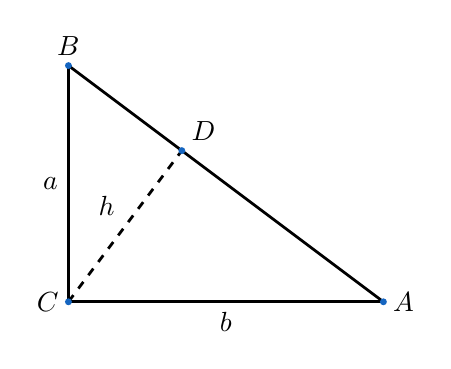
\begin{tikzpicture}[]

\coordinate[label=left:$C$] (C) at (0,0);
\coordinate[label=above:$B$] (B) at (0,3);
\coordinate[label=right:$A$] (A) at (4,0);
\coordinate[label=above right:$D$] (D) at (1.44,1.92);

\tkzMarkRightAngle[line width=1pt](A,C,B);
\tkzMarkRightAngle[line width=1pt](C,D,A);

\draw [line width=1pt] (C) to [edge label=$a$] (B);
\draw [line width=1pt] (A) to [edge label=$b$] (C);
\draw [line width=1pt] (A)-- (B);
\draw [line width=1pt,dash pattern=on 3pt off 3pt] (C) to [edge label=$h$] (D);

\foreach \p in {A,B,C,D}
	\fill[fill=rvwvcq,thick] (\p) circle (1.25pt);
\end{tikzpicture}
\end{wrapfigure}
\indent 根据勾股定理和面积关系, 可以推出:
\begin{align*}
ab &= ch \\
a^2b^2 &= c^2h^2\\
\frac{1}{h^2} &= \frac{c^2}{a^2b^2}=\frac{a^2+b^2}{a^2b^2}\\
\frac{1}{h^2} &= \frac{1}{a^2} + \frac{1}{b^2}
\end{align*}
这意味着当斜边上的垂足上有一个单位亮度的灯时, 感光元件接收的光强等于两个直角顶点上各有一个单位亮度灯时的光强.

现在假定感光元件位于原点 $ O $ 处, 一个小圆的圆心在 $ y $ 轴上, $ OA $ 为直径, 直径是 $ 2/\pi $, 周长为 2. 点 $ A $ 处有一个灯, 则 $ O $ 点的亮度为 $ \pi^2/4 $. 

在小圆外面画一个稍大一点的圆, 直径是小圆的两倍, 两圆内切于 $ O $ 点, 过点 $ A $ 作小圆的切线, 与大圆交于 $ B, C $ 两点. 点 $ OBC $ 构成直角三角形, $ BC $ 是斜边, $ A $ 是斜边上的垂足, 对 $ O $ 点而言, 在 $ B, C $ 两点上各放一个灯, 和在 $ A $ 点放一个灯的亮度是一样的. 

继续在大圆外面画一个更大的圆, 直径是前一个圆的两倍, 为 $ 8/\pi $, 同样与上一个圆相切于 $ O $ 点. 过新的大圆圆心分别作过 $ B $ 和 $ C $ 的直径, 两直径的端点分别是 $ D, E, F, G $, 容易证明这 4 个点平分了圆周. 考虑过 $ C $ 点的直径 $ FD $, $ OFD $ 三点构成直角三角形, $ \angle FOD $ 是直角. 另一方面, $ \angle FCO $ 是第二个圆的直径所对的圆周角, 从而 $ OC $ 是 $ FD $ 上的高. 于是对于 $ O $ 来说, $ C $ 点有一个灯, 等价于 $ F $ 和 $ D $ 上各有一个灯. 同理, $ B $ 点有一盏灯等价于 $ E $ 和 $ G $ 各有一盏灯, 所以 $ DEFG $ 的亮度之和等于 $ A $ 的亮度.

\begin{figure*}[htbp]
\centering
\definecolor{wrwrwr}{rgb}{0.3803921568627451,0.3803921568627451,0.3803921568627451}
\definecolor{rvwvcq}{rgb}{0.08235294117647059,0.396078431372549,0.7529411764705882}
\subfigure{
\begin{minipage}[b]{0.48\linewidth}
\centering
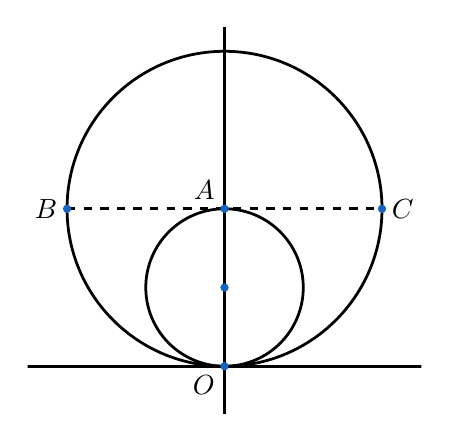
\begin{tikzpicture}[scale=2]
\clip(-1.25,-0.3) rectangle (1.25,2.15);
\coordinate[label=below left:$O$] (O) at (0,0);
\coordinate (C1) at (0,0.5);
\coordinate[label=above left:$A$] (A) at (0,1);
\coordinate[label=left:$B$] (B) at (-1,1);
\coordinate[label=right:$C$] (C) at (1,1);
\draw [line width=1pt] (A) circle (1cm);
\draw [line width=1pt] (C1) circle (0.5cm);
\draw [line width=1pt] (-2.2,0)--(3.1,0);
\draw [line width=1pt] (0,-0.7) -- (0,3.18);
\draw [line width=1pt,dash pattern=on 3pt off 3pt] (B)-- (C);
\foreach \p in {A,B,C,C1,O}
	\fill[fill=rvwvcq,thick] (\p) circle (0.75pt);
\end{tikzpicture} 
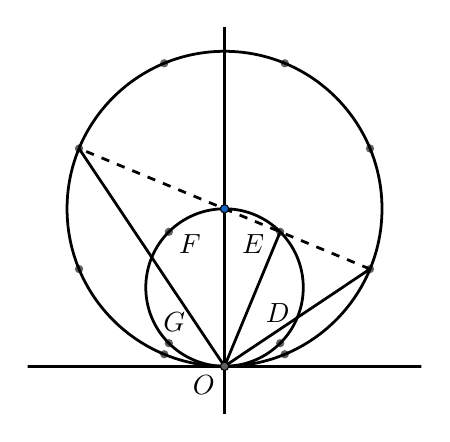
\begin{tikzpicture}[scale=2]
\clip(-1.25,-0.3) rectangle (1.25,2.15);
\coordinate[label=below left:$O$] (O) at (0,0);
\coordinate (C3) at (0,1);
\coordinate (C2) at (0,0.5);
\foreach \idx/\lab in {1/P1,-1/P2,3/P3,-3/P4,5/P5,-5/P6,7/P7,-7/P8} {
	\coordinate (\lab) at ({0 + 1*cos(270+\idx*22.5)},{1 + 1*sin(270+\idx*22.5)});
	\fill[fill=wrwrwr,thick] (\lab) circle (0.75pt);
}
\foreach \idx/\lab in {1/D,-1/G,3/E,-3/F} {
	\coordinate (\lab) at ({0 + 0.5*cos(270+\idx*45)},{0.5 + 0.5*sin(270+\idx*45)});
	\fill[fill=wrwrwr,thick] (\lab) circle (0.75pt);
}
\draw [line width=1pt] (C3) circle (1cm);
\draw [line width=1pt] (C2) circle (0.5cm);
\draw [line width=1pt] (-2.2,0)--(3.1,0);
\draw [line width=1pt] (0,-0.7) -- (0,3.18);
\draw (0.2,0.46) node[anchor=north west] {$D$};
\draw (0.05,0.9) node[anchor=north west] {$E$};
\draw (-0.35,0.9) node[anchor=north west] {$F$};
\draw (-0.45,0.4) node[anchor=north west] {$G$};
\draw [line width=1pt,dash pattern=on 3pt off 3pt] (P3)-- (P6);
\draw [line width=1pt] (P6) -- (O)-- (P3);
\draw [line width=1pt] (O) -- (E);
\draw [fill=rvwvcq] (0,1) circle (0.75pt);
\draw [fill=wrwrwr] (0,0) circle (0.75pt);
\end{tikzpicture}
\end{minipage}}
\subfigure{
\begin{minipage}[b]{0.48\linewidth}
\centering
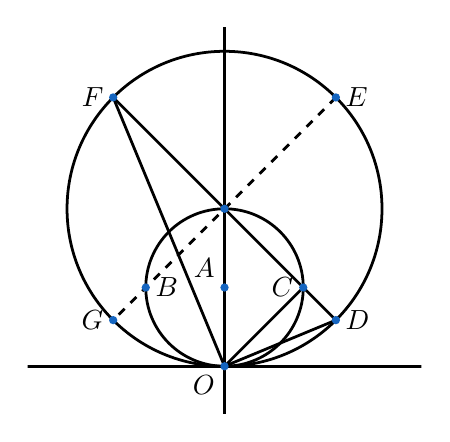
\begin{tikzpicture}[scale=2]
\clip(-1.25,-0.3) rectangle (1.25,2.15);
\def\xx{0.7071067811865475}
\coordinate[label=below left:$O$] (O) at (0,0);
\coordinate[label=right:$B$] (B) at (-0.5,0.5);
\coordinate[label=left:$C$] (C) at (0.5,0.5);
\coordinate[label=135:$A$] (A) at (0,0.5);
\coordinate[label=right:$D$] (D) at (\xx,1-\xx);
\coordinate[label=right:$E$] (E) at (\xx,1+\xx);
\coordinate[label=left:$F$] (F) at (-\xx,1+\xx);
\coordinate[label=left:$G$] (G) at (-\xx,1-\xx);
\coordinate (C2) at (0,1);
\draw [line width=1pt] (C2) circle (1cm);
\draw [line width=1pt] (A) circle (0.5cm);
\draw [line width=1pt] (-2.2,0)--(3.1,0);
\draw [line width=1pt] (0,-0.7) -- (0,3.18);
\draw [line width=1pt,dash pattern=on 3pt off 3pt] (E)-- (G);
\draw [line width=1pt] (F)-- (D);
\draw [line width=1pt] (F)-- (O);
\draw [line width=1pt] (O)-- (D);
\draw [line width=1pt] (O)-- (C);
\foreach \p in {A,B,C,C2,O,E,F,G,D}
	\fill[fill=rvwvcq,thick] (\p) circle (0.75pt);
\end{tikzpicture} 
\begin{tikzpicture}[line cap=round,line join=round,>=triangle 45,x=1cm,y=1cm,scale=2]
\clip(-1.25,-0.3) rectangle (1.25,2.15);
\coordinate[label=below left:$O$] (O) at (0,0);
\coordinate (C4) at (0,16);
\foreach \idx/\lab in {1/P1,-1/P2,3/P3,-3/P4,5/P5,-5/P6,7/P7,-7/P8} {
	\coordinate (\lab) at ({0 + 16*cos(270+\idx*0.5)},{16 + 16*sin(270+\idx*0.5)});
  	\draw [line width=1pt,dash pattern=on 3pt off 3pt] (C4) -- (\lab);
	\fill[fill=wrwrwr,thick] (\lab) circle (0.75pt);
}
\draw [line width=1pt] (-3.8,0) -- (3.4,0);
\draw [line width=1pt] (0,-0.58) -- (0,3.3);
\draw [line width=1pt] (C4) circle (16cm);
\end{tikzpicture}
\end{minipage}}
\end{figure*}
继续在外面画一个更大的圆, 直径是上一个圆的两倍, 过 $ DEFG $ 作大圆的直径, 得到大圆的 8 个等分点, 类似的, 如果这 8 个点上各放一个灯, 它们的亮度之和与 $ A $ 点的亮度是一样的. 另外注意到这一系列圆上, 等分点之间的弧长都是 2.

这个过程一直进行下去, 随着圆越来越大, 曲率越来越小, 得到的等分点在极限情况下都会落在 $ x $ 轴上, 对应的坐标分别是 $ \pm1, \pm3, \cdots $. 这些灯的亮度之和依然是 $ \pi^2/4 $. 即:
\[ \frac{1}{1^2} + \frac{1}{3^2} + \frac{1}{5^2} + \cdots = \frac{\pi^2}{8}. \]
经过简单的代换:
\begin{align*}
\zeta(2) - \frac{1}{4}\zeta(2) &= \left( \frac{1}{1^2} + \frac{1}{2^2} + \frac{1}{3^2} + \cdots \right) - \left( \frac{1}{2^2} + \frac{1}{4^2} + \frac{1}{6^2} + \cdots \right)\\
\frac{3}{4}\zeta(2) &= \frac{1}{1^2} + \frac{1}{3^2} + \frac{1}{5^2} + \cdots = \frac{\pi^2}{8} \\
\zeta(2) &= \frac{\pi^2}{6}
\end{align*}


\newpage
%------------------------------------------------------------------------------%
\section{Leibniz级数与$\pi$}

证明: $$ 1 - \frac{1}{3} + \frac{1}{5} - \frac{1}{7} + \cdots = \frac{\pi}{4} $$.

\subsection{中国剩余定理}
假设整数 $ m_1, m_2, \cdots, m_n $ 两两互质, 则对任意的整数 $ a_1, a_2, \cdots, a_n $, 下面的方程组都有解: 
\begin{equation*}
\ \begin{cases}
x\equiv a_{1} & \pmod{m_1}\\
x\equiv a_{2} & \pmod{m_2}\\
\cdots  & \\
x\equiv a_{n} & \pmod{m_n}
\end{cases}
\end{equation*}
并且通解可以用如下方式构造得到: 

设 $ M = m_1\times m_2\times\cdots\times m_n = \prod_{i=1}^{n}{m_i} $, 并设 $ M_i = M / m_i $ 是除了 $ m_i $ 以外的 $ n - 1 $ 个数的乘积, 设 $ t_i = M_i^{-1} $ 是 $ M_i $ 模 $ m_i $ 的逆元: $ M_it_i \equiv 1 \pmod{m_i} $, 则上述方程组的通解为: $ x = x_0 + kM, k\in \mathbb{Z} $, 其中 $$ x_0 = a_1t_1M_1 + a_2t_2M_2\cdots + a_nt_nM_n $$ 是一个特解.

因为当 $ i \neq j $ 时, $ m_i $ 与 $ m_j $ 互质, 则 $ m_i $ 和 $ M_i $ 也互质. 所以 $ M_i $ 模 $ m_i $ 的逆元是存在的, $ a_it_iM_i \equiv a_i \pmod{m_i} $. 另一方面, 当 $ i \neq j $ 时, $ m_i $ 是 $ M_j $ 的因数, 所以 $ a_jt_jM_j \equiv 0 \pmod{m_i}) $. 于是 $ x_0 $是满足方程组的一个解. 

如果有两个解 $ x_1 $ 和 $ x_2 $ 都满足上面的方程组, 对于任意的 $ i\in\{1, 2, \cdots, n\} $, 都有 $ x_1 - x_2 \equiv 0 \pmod{m_i} $, 说明 $ m_i $ 整除 $ x_1 - x_2 $, 而 $ m_1, m_2, \cdots, m_n $ 两两互质, 说明 $ M $ 也整除 $ x_1 - x_2 $, 即任意两个解之差都是 $ M $ 的倍数. 这就证明了上述通解的形式包含了所有的解.

\subsection{欧拉函数}
对正整数 $ x $, 定义欧拉函数 $ \phi(x) $ 为小于或等于 $ x $ 的正整数中, 与 $ x $ 互质的数的数目. 
有以下性质:

\noindent (1) 对任意素数 $ p $, $ \phi(p) = p - 1 $, 这是显然的.

\noindent (2) 对任意素数 $ p $, $ \phi(p^k) = p^k - p^{k-1} = p^k(1-1/p) $. 

这是因为不超过 $ p^k $ 的数中, 与 $ p^k $ 具有相同的因数的数集合为 $ \{ p, 2\times p, \cdots, p^{k-1}\times p \} $, 共 $ p^{k-1} $ 个. 

\noindent (3) 对于任意的素数 $ p, q $, 若 $ p \neq q $, 则 $ \phi(p^mq^n) = \phi(p^m)\phi(q^n) $. 

考虑定义, 不超过 $ p^mq^n $ 的数中, 与 $ p^mq^n $ 不互素的数有 $ p $ 的倍数: $ \{p,2p,\cdots,p^mq^n\} $ 和 $ q $ 的倍数 $ \{q,2q,\cdots,p^mq^n\} $. 两个集合中重复的元素是 $ \{pq, 2pq, \cdots, p^mq^n \} $, 则 $ \phi(p^mq^n) = p^mq^n - p^{m-1}q^{n} - p^{m}q^{n-1} + p^{m-1}q^{n-1} = \phi(p^m)\phi(q^n) $.

\noindent (4) 由上一条容易推断: 对于互质的两个数 $ a, b $, 有 $ \phi(ab) = \phi(a)\phi(b) $.

\noindent (5) 设 $ p_1, p_2, \cdots, p_n $ 为 $ x $ 的所有质因数, 则: $$ \phi(x) = x\prod_{i=1}^{n}{(1-\frac{1}{p_i})} $$.

	对 $ x $ 分解质因数: $ x = p_1^{k_1}p_2^{k_2}\cdots p_n^{k_n} $, 根据 (2) 和 (3), $ \displaystyle \phi(x) = \prod_{i=1}^n\left[p_i^{k_i}(1-\frac{1}{p_i})\right] $, 即得.

\subsection{欧拉定理和费马小定理}

\noindent 欧拉定理: 若 $ a $ 和 $ n $ 互质, 则 $ a^{\phi(n)} \equiv 1 \pmod{n} $. 

\noindent 证明: 设小于 $ n $ 且和 $ n $ 互质的数的集合为 $ \{ X_1, X_2, \cdots, X_m \} $, 其中 $ m = \phi(n) $.

考虑集合 $ \{ aX_1, \cdots, aX_m\} $, 如果 $ aX_i \equiv aX_j \pmod{n} $, 则 $ a(X_i-X_j) \equiv 0 \pmod{n} $, 而 $ n $ 与 $ a $ 互质, 所以 $ X_i - X_j $ 整除 $ n $, 再由 $ X_i, X_j \in [1,n] $, 于是只能是 $ X_i = X_j $. 反过来看, 若 $ X_i \neq X_j $, 则 $ aX_i \neq aX_j $. 所以集合 $ \{aX_i\} $ 也有 $ m $ 个不同元素, 且都与 $ n $ 互质 ( 这是因为 $ a $ 和 $ X_i $ 都与 $ n $ 互质).
 
这意味着集合 $\{aX_i\}$ 和集合 $\{X_i\}$ 在模 $ n $ 下是相同的. 将它们的所有元素乘起来:
$$ X_1\cdot X_2\cdots X_m \equiv aX_1\cdot aX_2\cdots aX_m \pmod{n} $$ 
亦即 $ (a^m - 1)\prod{X_i} \equiv 0 \pmod{n} $.

因为 $ X_i $ 和 $ n $ 互质, 所以 $ a^m - 1 \equiv 0 \pmod{n} $, 或 $ a^{\phi(n)} \equiv 1 \pmod{n} $.

~

\noindent 费马小定理: 若 $ a $ 和素数 $ p $ 互质, 则 $ a^{p-1} \equiv 1 \pmod{p} $. 这是欧拉定理的特例.

\subsection{有限差分}

命题: 序列 $ 1^k, 2^k, 3^k, \cdots, n^k, \cdots $ 的 $ k $ 阶差分序列全都等于 $ k! $. 其中 $ i $ 阶差分序列的定义为 $ D^{(i)}_n = D^{(i-1)}_{n+1} - D^{(i-1)}_n, \ n\in\mathbb{N} $; $ 0 $ 阶差分就是原序列: $ D^{(0)}_n = x_n $.

用归纳法可证明. 首先当 $ k = 1 $ 时, 差分序列为 $ 1, 1, \cdots $, 结论成立.

假设命题对于任意 $ k = 1, 2, \cdots, m - 1 $ 都成立, 考虑 $ k = m $, 为了算 $m$ 阶差分, 先算一阶的. 它的一阶差分序列通项为 
$$ D^{(1)}_n = (n+1)^{m} - n^m = 1 + C_m^1n + C_m^2n^2+\cdots+C_m^{m-1}n^{m-1} .$$ 

先考虑前 $ m - 2 $ 项, 接下来要做 $ m - 1 $ 次差分, 由归纳假设, $ n $ 的一次方项经过一次差分变成 $ 1!C_m^1 $, 平方项经过2次差分变成 $ 2!C_m^2 $, 等等, 它们都是常数, 到 $ m - 1 $ 次差分的时候都变成了 $ 0 $; 而最后一项经过 $ m - 1 $ 次差分变成了 $ (m-1)!C_m^{m-1} = m! $. 

说明当 $ k = m $ 的时候也成立. 所以命题得证.

\subsection{$4k+1$型素数的平方和分解}

\noindent 定理: 如果素数 $ p $ 模 $ 4 $ 余数是 $ 1 $, 则存在唯一一对整数 $a,b$, 使得 $ p = a^2 + b^2 $.

先证明存在性, 这里介绍欧拉的方法, 分为 5 个步骤.

\noindent (1) 若 $ x,y $ 都是两个整数的平方和, 则它们的乘积也是两个整数的平方和.

证明: 设 $ x = a^2+b^2, y = p^2+q^2 $, 则 \[ xy = (a^2+b^2)(p^2+q^2)=(ap+bq)^2+(aq-bp)^2 .\]

~

\noindent (2) 若 $ x,y $ 都是两个整数的平方和, $ y $ 是素数, 且 $ y $ 整除 $ x $, 则 $ x/y $ 也是两个整数的平方和.

证明: 设 $ x = a^2+b^2, y = p^2+q^2 $, 考虑下面的关系:
\begin{align*} 
z = (pb-aq)(pb+aq) & = p^2b^2-a^2q^2 \\
	& = p^2(a^2+b^2)-a^2(p^2+q^2)\\
	& =p^2x-a^2y.
\end{align*}

因为 $ y $ 整除 $ x $, 则 $ y $ 也整除 $ z $. 又因为 $ y $ 是素数, 所以 $ y $ 一定整除 $ pb-aq $ 或 $ pb + aq $. 先假设 $ y $ 整除 $ pb-aq $, 观察到
\[ xy = (a^2+b^2)(p^2+q^2)=(ap+bq)^2+(aq-bp)^2 ,\]
两边除以 $ y^2 $:
\[ \frac{x}{y} = \left(\frac{ap+bq}{y}\right)^2+\left(\frac{bp-aq}{y}\right)^2 .\]

$ y $ 整除 $ pb-aq $ 和 $ x $, 等式两边都是整数, 所以 $ y $ 也必须整除 $ ap+bq $. 这里 $ x/y $ 就已经是两个整数的平方和了.

如果$ y $ 整除 $ pb+aq $, 类似的有
\[ xy = (a^2+b^2)(p^2+q^2)=(aq+bp)^2+(ap-bq)^2 ,\]
也能成立.

~

\noindent (3) 若 $ x $ 是两个整数的平方和, $ y $ 整除 $ x $, 且 $ y $ 不能表示成两个整数的平方和, 则 $ x/y $ 也存在一个因子无法写成两整数平方和.

证明: 对 $ x/y $ 做素因数分解: $ x/y=p_1p_2\cdots p_n $. 如果所有的 $p_i$ 都能写成两整数的平方和, 反复应用上面第(2)条, 可以推出 $ x/p_1 $ 能写成两个整数平方和, $ x/(p_1p_2) $ 也能, 等等, 一直到 $ x/(p_1p_2\cdots p_n)=y $ 也是两个整数平方和.这与条件矛盾.

~

\noindent (4) 若 $ a,b $ 互素, 则 $ a^2+b^2 $的所有因数都能表示成两个整数平方之和.

证明: 如果 $ a^2 + b^2 $ 是素数, 命题已经得证. 假设 $ q $ 是 $ a^2+b^2 $ 的任一因数. $q=2$时也显然成立. 下面考虑 $ q > 2 $ 的情况.

选取非负整数 $ m $ 和 $ n $, 使得 $mq$ 和 $nq$ 分别是距离 $a$和$b$的最近的 $q$的倍数. 有没有可能 $q$是偶数且 $|mq-a| = q/2 $ 呢? 如果是这样, 则 $q/2$ 一定是 $ a $ 的因数, 而 $ q $ 是 $a^2+b^2$ 的因数, 所以$ q/2 $ 也是 $a^2+b^2$ 的因数, 这就说明 $q/2$ 也是 $b$ 的因数, 这与 $ a,b $ 互素矛盾.

令 $ c=mq-a, d=nq-b$. 则 $ |c| < q/2, |d| < q/2 $. 
\[ a^2 + b^2 = (mq-c)^2+(nq-d)^2 = Aq+(c^2+d^2) ,\]
这里 $ A $ 是一个合适的整数.

因为 $q$ 是 $a^2+b^2$的因数, 上式表明 $q$ 也是 $ ( c^2 + d^2 ) $ 的因数. 于是令 $ c^2 + d^2 = qr $, 并设 $ c,d $ 的最大公约数为 $ g $, 则可知 $ g $ 与 $ q $ 互质. (否则由 $ a=c+mq $ 和 $ b=d+nq $, $gcd(g,q)$ 也能整除 $a$ 和 $b$, 与 $a,b$ 互素矛盾.)

再由 $ g^2 $ 整除 $ qr $, 得 $ g^2 $ 是 $ r $ 的因数. 设 $ r = sg^2, e=c/g, f=d/g $. 则
\[ qs = \frac{qr}{g^2}=e^2+f^2\leq c^2+d^2 < (\frac{q}{2})^2 + (\frac{q}{2})^2 = \frac{q^2}{2} \] 
不等式两边约去 $ q $ 得到 $ s < q/2 $. 

因为 $ qs $ 是两整数平方和, 如果 $ q $ 不能写成两整数平方和, 则根据上面第(3)条, $ s $ 存在一个因数 $ q_1 $ 不能写成两整数平方和, $ q_1 \leq s < q/2 < q $. 现在有 $ e,f $ 互素, $ q_1 $ 是 $ e^2+f^2 $ 的因数, 重复上面的构造过程 ( $a,b,q$ 分别换成 $e,f,q_1$), 将得到 $q_2 < q_1$, 反复构造将得到一个严格递减的无穷正整数序列, 这是不可能的. 所以 $ q $ 可以写成两整数平方和.

~

\noindent (5) 任意 $ 4n + 1 $ 形式的素数都能写成两个整数的平方和.

证明: 设 $ p = 4n + 1 $, 由费马小定理, 对任意的 $ a $, 都有 $ a^{4n} \equiv 1 \pmod{p} $. 令 $ a $ 取 $ 1, 2, \cdots, 4n $, 则序列 $ S = \left[2^{4n}-1^{4n}, \cdots, (4n)^{4n}-(4n-1)^{4n} \right] $ 中的每一项都可以被 $ p $ 整除. 分析它们的通项: \[ a^{4n}-b^{4n}=(a^{2n}+b^{2n})(a^{2n}-b^{2n}),\] 
其中 $ a=b+1 $, 于是 $a,b$ 互素.

因为 $p$ 是素数, 所以 $p$ 整除 $ a^{2n}+b^{2n} $ 或 $ a^{2n}-b^{2n} $. 如果上述序列 $ S $ 的 $ 4n-1 $ 项中有一项是 $p$ 整除 $ a^{2n}+b^{2n} $, 根据上面的第(4)条, 可知 $p$ 可以表示成两整数的平方和. 

反之, 如果全部 $ 4n-1 $ 种情况下都是 $p$ 整除 $ (b+1)^{2n}-b^{2n} $, 我们从有限差分的性质推出这是不可能的.
考虑序列 $ 1^{2n}, 2^{2n}, \cdots, (4n)^{2n} $, 根据假设, 它的一阶差分都是 $p$ 的倍数, 从而更高阶的差分也都是 $ p $ 的倍数. 特别地, 取 $ 2n $ 阶差分, 它每一项都等于 $ (2n)! $, 因为 $ p $ 是素数, $ 2n < 4n + 1 = p $, 说明 $(2n)!$ 不可能被 $p$ 整除, 矛盾.

~

下面证明$4k+1$型素数的平方和分解的唯一性.

如果存在两种分解方式 $ p = a^2+b^2=c^2+d^2 $, 不妨设 $a,b,c,d $ 都是正整数, 注意到
\begin{align*} 
p^2=(a^2+b^2)(c^2+d^2) & =(ac+bd)^2+(ad-bc)^2 \\ & =(ac-bd)^2+(ad+bc)^2 .\end{align*}
此外由 $ (p-a^2)d^2=(p-c^2)b^2 $, 可得 $ p(d^2-b^2)=(ad-bc)(ad+bc) $.

$ p $是素数, 若 $p$ 整除 $ ad-bc$, 由 $p^2=(ac+bd)^2+(ad-bc)^2$, 知 $ (ad-bc)^2 = p^2-(ac+bd)^2 < p^2 $, 从而 $ ad-bc=0 $. 于是 $ d^2=b^2 $, 说明两种分解方式是相同的.

若 $p$ 整除 $ad+bc$, 由 $p^2=(ac-bd)^2+(ad+bc)^2$ 知 $ (ad+bc)^2 = p^2 $, 从而 $ ac = bd $. 又易知 $a,b$ 互素, 所以 $ a $ 整除 $ d $ 且 $ b $ 整除 $ c $. 不难得到 $ a=d, b=c $.


\subsection{高斯整数和高斯素数}

高斯整数定义为复数集合 $ \mathbb{Z}\left[i\right] = \{ a + bi\ |\ a,b\in\mathbb{Z},\ i^2=-1\} $, 也就是复平面上的整点. 

同整数的素数分解一样, 高斯整数也有素数分解, 但不唯一. 考虑 $ z = x\cdot y $, 同时也有 $ z = (ix)\cdot(-iy) = (-x)\cdot(-y) = (-ix)\cdot(iy) $. 这 4 种分解方式本质上都是一样的.

再考虑共轭复数的分解. 如果 
$$ z = x\cdot y = (a+bi)(c+di) = (ac-bd)+i(ad+bc), $$ 则 $$ \bar{z} = (ac-bd)-i(ad+bc) = (a-bi)(c-di) = \bar{x}\bar{y}. $$ 这说明了共轭复数的分解存在一一对应关系.

观察 $ z\bar{z}= (x\bar{x})(y\bar{y}) $, 左边是一个实整数, 右边每一对共轭因子的乘积也是实整数. 我们对 $ z $ 的模长平方做素数分解, 再将所得的每个素因子分解成一对共轭复数的乘积, 就可以得到 $ z\bar{z} $ 的高斯素数分解. 每对因子 $ x $ 和 $ \bar{x} $ 种有且只有一个能被 $ z $ 整除, 只要试一下就知道该取哪一个作为 $ z $ 的因子.

素的实整数 $ p $ 能否分解成共轭复数的乘积? 等价于求整数 $ a, b $ 满足 $ a^2 + b^2 = p $.

若 $ p = 2 $, 有 $ 2 = 1^2 + 1^2 = (1+i)(1-i) $.

若 $ p = 4k + 3 $, 先考虑 $ a, b \bmod{4} $ 的结果, 可能有 $\{0, 1, 2, 3\} $ 这些情况; 而 $ a^2, b^2 \bmod{4} $ 只有 $ \{0, 1\} $ 两种情况; $ a^2 + b^2 \bmod{4} $ 的取值范围为 $ \{0,1,2\} $. 于是 $ p = 4k + 3 $ 类型的素数无法进一步分解.

若 $ p = 4k + 1$, 存在唯一的分解方式.

\subsection{半径为 $ \sqrt{n} $ 的圆周上的整点个数}

考虑圆心在原点, 半径为 $ R $ 的圆, 当 $ R $ 足够大时, 圆内的整点数量和圆的面积趋近于相等. 因此如果知道圆内整点数量和半径 $ R $ 的关系, 就能求出 $ \pi $ 的一种逼近方式.

整点到原点的距离平方都是整数, 为了数出圆内整点个数, 可以将它们按同心圆归类. 例如, 半径为 $ 1 $ 的圆上有 $ 4 $ 个整点, 而半径为 $ \sqrt{5} $ 的圆上有 $ 8 $ 个, 半径 $ 5 $ 的圆上有 $ 12 $ 个. 只要数清楚半径为 $ \sqrt{n} $ 上有多少整点. 这等价于求 $ x^2+y^2 = n $ 的整数解个数, 或者说求 $ n $ 在复数域上的分解 $ n = (x+iy)(x-iy) $ 的个数.

先考虑 $ n $ 是素数的情况, 此时仅当 $ n $ 是 $ 4k + 1 $ 的形式才有唯一的平方和分解: $ n = a^2 + b^2 = (a+bi)(a-bi) $, 取其中这对共轭因子的任意一个, 将它乘以 $ \pm 1 $ 和 $ \pm i $, 可以得到 8 个不同的复数, 对应了 $ (\pm a, \pm b), (\pm b, \pm a) $ 共 $8$ 个整点. 特别的, 当 $ n = 2 $ 时, $ a = b = 1 $, 这 $8$ 个点有一半是重复的.

再考虑 $ n $ 是素数的整数次幂的情况: $ n = p^m $. 当 $ p = 4k + 3 $ 时, 只有 $ m $ 是偶数才存在分解 $ n = (p^\frac{m}{2})^2 + 0^2 $, 对应两坐标轴上的 $4$ 个整点. 当 $ p = 4k + 1 = a^2+b^2 $ 时, $ n = (a+bi)^m(a-bi)^m $, 需要在这 $ m $ 对共轭因子中凑出两对共轭的乘积 $ (x\pm iy) $, 所以每一对因子其中一个贡献给 $(x+iy)$, 另一个贡献给 $(x-iy)$. 这些因子一共可以乘出 $m+1$ 个不同的乘积 $ (x\pm iy) $, 分别是 $(a+bi)^l(a-bi)^{m-l} $, $ 0 \le l \le m $. 这些乘积经过 $ \pm 1 $ 和 $ \pm i $ 旋转后有 $ 4(m+1) $ 个整点. 特别的, 当 $ p = 2 $ 时, 仍然存在大量重复的点, 实际上不同的点只有坐标轴上的 $4$ 个.

最后考虑一般的情况, 对 $ n $ 做素数分解, 设素因数 $ p_i $ 对应的指数为 $ m_i $, 则 $ p_i^{m_i} $ 可以生成 $ 0, 1, m+1 $ 种不同的 $(x_i+iy_i)$, 取决于 $ p_i $ 和 $ m_i $ 的取值 ( 注意这里去掉了乘以 $ \pm 1 $ 和 $ \pm i $ 的旋转对称的情况 ). 不同素因数分解出来的 $(x_i+iy_i)$ 可以自由组合, 不会乘出来重复的数, 所以, $ n $ 分解出来的高斯整数是各个不同因数对应的分解个数乘起来.

% \subsection{$\chi$ 函数}

现定义一个正整数上的函数 $ \chi(n) $ : 
\begin{equation*}
\chi(n) = \begin{cases}
0,\ \ if \ n \equiv 0 \pmod{2}\\
1,\ \ if \ n \equiv 1 \pmod{4}\\
-1,\ \ if \ n \equiv 3 \pmod{4}
\end{cases}
\end{equation*}
不难验证 $ \chi(mn) = \chi(m)\chi(n) $ 对任意正整数 $ m, n $ 都成立.

回到圆周上的整点问题, 当 $ n $ 是素数的整数次幂, $ n=p^m=(x+iy)(x-iy) $ 的分解出来的(共轭)复数有 $ F(p,m) = 1 + \chi(p) + \chi(p^2) + \cdots + \chi(p^m) $ 这么多个. ( 同样忽略了旋转对称.) 可以验证, 对于 $ p = 2 $, $ p = 4k+1 $, 和 $ p=4k+3 $ 型的素数都是成立的. 

于是对于 $ n = \prod{p_i^{m_i}} $, 分解出来的高斯整数个数是 $ G(n) = \prod{F(p_i,m_i)} $. 可以把这个乘积展开, 并利用 $ \chi $ 函数的可乘性. 则 $ G(n) = \sum_{d|n}{\chi(d)} $, 也就是对 $ n $ 的所有因数求 $ \chi $ 函数值, 再加起来. 

\subsection{半径 $ R $ 的圆内的整点个数}
令 $ n $ 从 $ 1 $ 取到 $ R^2 $, 对上面的结论分别求 $ G(n) $, 并求和, 就得到半径 $ R $ 的圆内的整点个数. 现在观察不同的 $ \chi $ 函数出现了多少次.
\begin{align*}
G(1) &= \chi(1) \\
G(2) &= \chi(1) + \chi(2) \\
G(3) &= \chi(1) + \chi(3) \\
G(4) &= \chi(1) + \chi(2) + \chi(4) \\
G(5) &= \chi(1) + \chi(5) \\
G(6) &= \chi(1) + \chi(2) + \chi(3) + \chi(6)\\
\cdots
\end{align*}

对每个 $d$, $ \chi(d) $ 都会在 $ G(kd) $ 里都会出现, 也就是每隔 $d$ 行出现一次.
于是 $ R^2 $ 行里出现次数为 $ R^2/d $.
将他们加起来, 并考虑 4 倍的旋转对称:
\[ \pi R^2 \approx 4\sum_{n=1}^{R^2}{G(n)} = 4R^2\left( 1 + \frac{\chi(2)}{2} + \frac{\chi(3)}{3} + \cdots + \frac{\chi(R^2)}{R^2} \right) .\]

把 $ \chi $ 函数的值代进去, 并令 $ R $ 趋于无穷, 约等于就变成等于:
\[ \frac{\pi}{4} = 1 - \frac{1}{3} + \frac{1}{5} -\frac{1}{7} + \cdots \]

\newpage
%------------------------------------------------------------------------------%

\section{Wallis 乘积}

Wallis 乘积公式: \[ \frac{\pi}{2} = \frac{2}{1}\cdot\frac{2}{3}\cdot\frac{4}{3}\cdot\frac{4}{5}\cdot\frac{6}{5}\cdot\frac{6}{7}\cdots \]

先证明一个引理: 单位圆上有 $ N $ 个等分点, 其中相邻两个点之间的圆弧的中点到所有这些等分点的直线距离的乘积恒等于 $ 2 $; 而某个等分点到其余等分点的直线距离的乘积等于 $ N $.

考虑复数域上的方程 $x^N-1=0 $ , 它有 $ N $ 个复数根 $ x_k = e^{k\omega i}$, 其中 $ \omega = \frac{2\pi}{N}, k=0,1,\cdots,N-1 $. 这些根正好是复平面上单位圆的 $ N $ 个等分点. 所以原方程写成根式的形式: \[ x^N - 1 = (x - x_0)(x - x_1)\cdots(x-x_{N-1}) .\] 它对于任意的复数 $ x $ 当然也是成立的. 设 $ f \in (0,1) $, 取一点 $ X_f =  e^{f\omega i} $, 对应 $ x_0 $ 到 $ x_1 $ 之间占比为 $ f $ 的复数点. 对它取 $ N $ 次方自然是得到整个圆周占比为 $ f $ 的复数点 $e^{2\pi fi}$ . 代入上面的公式, 并对两边取模得到:
\[ || X_f^N-1 || = ||(X_f-x_0)||\cdot||(X_f - x_1)||\cdots||(X_f-x_{N-1})|| .\]

观察左边是复数 $e^{2\pi fi}$ 到 $ 1 $ 的距离, 右边是 $ N $ 个距离的乘积. 将 $\displaystyle f = \frac{1}{2} $ 代入, 左边是 $ 2 $, 右边是 $ x_0 $ 到 $ x_1 $ 之间圆弧的中点到其他各个复数根时间的距离之积. 引理第一条得证.

\begin{figure*}[htbp]
\definecolor{ududff}{rgb}{0.30196078431372547,0.30196078431372547,1}
\definecolor{rvwvcq}{rgb}{0.08235294117647059,0.396078431372549,0.7529411764705882}
\definecolor{uuuuuu}{rgb}{0.26666666666666666,0.26666666666666666,0.26666666666666666}
\centering
\begin{minipage}[t]{0.49\linewidth}
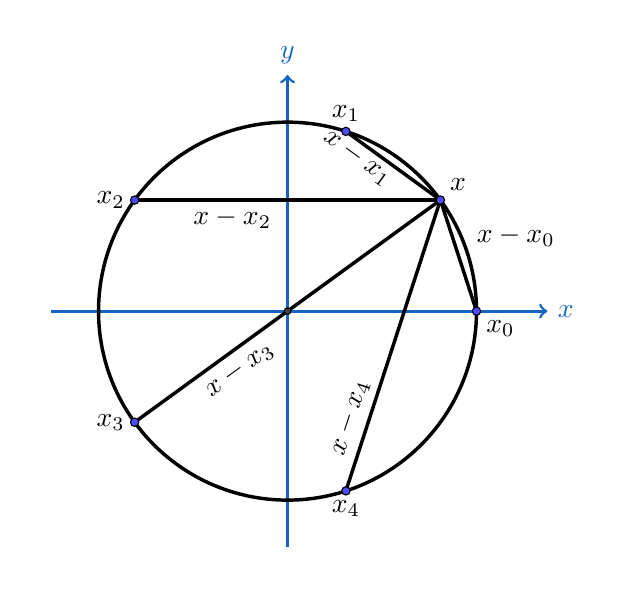
\begin{tikzpicture}[scale=0.6]
\coordinate[] (O) at (0,0);
\coordinate[label=below right:$x_0$] (A) at (4,0);
\coordinate[label=above:$x_1$] (B) at (1.2360679774997898,3.804226065180614);
\coordinate[label=left:$x_2$] (C) at (-3.2360679774997894,2.3511410091698925);
\coordinate[label=left:$x_3$] (D) at (-3.23606797749979,-2.351141009169892);
\coordinate[label=below:$x_4$] (E) at (1.2360679774997891,-3.8042260651806146);
\coordinate[label=above right:$x$] (X) at (3.23606797749979,2.3511410091698925);
\clip(-5.5,-5.5) rectangle (6.5,6.0);
\draw[rvwvcq,->,line width=1pt] (-5.0,0) -- (5.5,0) node[right] {$x$};
\draw[rvwvcq,->,line width=1pt] (0,-5.0) -- (0,5.0) node[above] {$y$};
\draw [line width=1.25pt] (O) circle (4cm);
\draw [line width=1.25pt] (A)-- (X);
\draw [line width=1.25pt] (X)-- (B);
\draw [line width=1.25pt] (X)-- (C);
\draw [line width=1.25pt] (X)-- (D);
\draw [line width=1.25pt] (X)-- (E);
\draw (3.8,2.0) node[anchor=north west] {$x-x_0$};
\draw (0.9,4.2) node[anchor=north west,rotate=-36] {$x-x_1$};
\draw (-2.2,2.38) node[anchor=north west] {$x-x_2$};
\draw (-2.1,-1.5) node[anchor=north west,rotate=36] {$x-x_3$};
\draw (0.6,-3.1) node[anchor=north west,rotate=72] {$x-x_4$};
\begin{scriptsize}
\draw [fill=uuuuuu] (O) circle (2pt);
\draw [fill=ududff] (A) circle (2.5pt);
\draw [fill=ududff] (B) circle (2.5pt);
\draw [fill=ududff] (C) circle (2.5pt);
\draw [fill=ududff] (D) circle (2.5pt);
\draw [fill=ududff] (E) circle (2.5pt);
\draw [fill=ududff] (X) circle (2.5pt);
\end{scriptsize}
\end{tikzpicture}
\end{minipage}
\begin{minipage}[t]{0.49\linewidth}
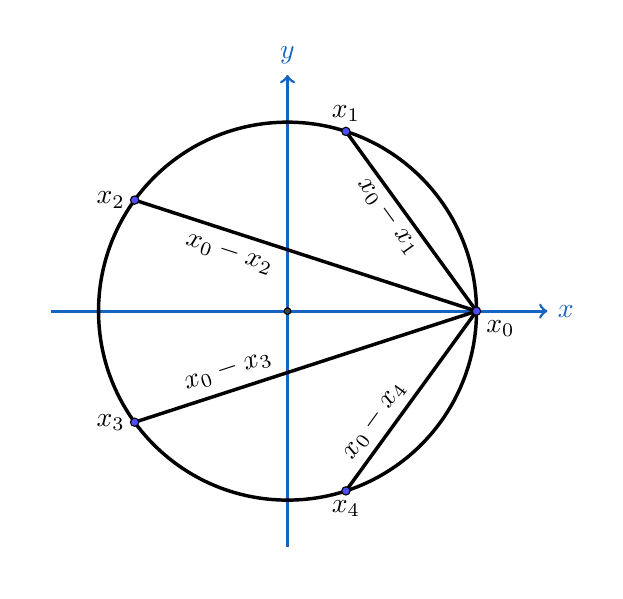
\begin{tikzpicture}[scale=0.6]
\coordinate[] (O) at (0,0);
\coordinate[label=below right:$x_0$] (A) at (4,0);
\coordinate[label=above:$x_1$] (B) at (1.2360679774997898,3.804226065180614);
\coordinate[label=left:$x_2$] (C) at (-3.2360679774997894,2.3511410091698925);
\coordinate[label=left:$x_3$] (D) at (-3.23606797749979,-2.351141009169892);
\coordinate[label=below:$x_4$] (E) at (1.2360679774997891,-3.8042260651806146);
\clip(-5.5,-5.5) rectangle (6.5,6.0);
\draw[rvwvcq,->,line width=1pt] (-5.0,0) -- (5.5,0) node[right] {$x$};
\draw[rvwvcq,->,line width=1pt] (0,-5.0) -- (0,5.0) node[above] {$y$};
\draw [line width=1.25pt] (O) circle (4cm);
\draw [line width=1.25pt] (A) -- (B);
\draw [line width=1.25pt] (A)-- (C);
\draw [line width=1.25pt] (A)-- (D);
\draw [line width=1.25pt] (A)-- (E);
\draw (1.8,3.2) node[anchor=north west,rotate=-54] {$x_0-x_1$};
\draw (-2.2,2.0) node[anchor=north west,rotate=-18] {$x_0-x_2$};
\draw (-2.5,-1.2) node[anchor=north west,rotate=18] {$x_0-x_3$};
\draw (0.8,-3.0) node[anchor=north west,rotate=54] {$x_0-x_4$};
\begin{scriptsize}
\draw [fill=uuuuuu] (O) circle (2pt);
\draw [fill=ududff] (A) circle (2.5pt);
\draw [fill=ududff] (B) circle (2.5pt);
\draw [fill=ududff] (C) circle (2.5pt);
\draw [fill=ududff] (D) circle (2.5pt);
\draw [fill=ududff] (E) circle (2.5pt);
\end{scriptsize}
\end{tikzpicture}
\end{minipage}
\end{figure*}

另一方面, 为了求出 $ x_0 = 1 $ 到其他根的距离之积, 对 $ x^N - 1 $ 做因式分解: \
\[ x^N-1 = (x-1)(1+x+x^2+\cdots+x^{N-1}) ,\]
于是
\[ ||x-x_1||\cdot||x-x_2||\cdots||x-x_{N-1}|| = \frac{||x^N-1||}{||x-1||} = || 1+x+x^2+\cdots+x^{N-1} || .\] 
把 $ x = 1 $ 代入上式, 左边是其中一个根到其他所有根的距离之积, 右边是 $ N $, 引理第二条也得证.

然后, 考虑两个点 $ A = 1, B = e^{\frac{1}{2}\omega i} $, 并记单位圆上 $ A $ 点逆时针方向的等分点为 $ x_1, x_2, \cdots $, 顺时针方向的点为 $ x_{-1}, x_{-2}, \cdots $. 计算下面的比值:
\[ P = \frac{||A-x_1||}{||B-x_1||} \frac{||A-x_{-1}||}{||B-x_{-1}||} \cdot \frac{||A-x_2||}{||B-x_2||} \frac{||A-x_{-2}||}{||B-x_{-2}||} \cdots \]

\begin{figure*}[htbp]
\definecolor{qqwuqq}{rgb}{0,0.39215686274509803,0}
\definecolor{ududff}{rgb}{0.30196078431372547,0.30196078431372547,1}
\definecolor{uuuuuu}{rgb}{0.26666666666666666,0.26666666666666666,0.26666666666666666}
\centering
\begin{tikzpicture}[cap=round,scale=3.0]
\coordinate[] (O) at (0,0);
\coordinate[label=below right:$A$] (A) at (4,0);
\coordinate[label=right:$B$] (B) at (3.9945181390182953,0.20934382497177534);
\coordinate[label=right:$x_1$] (C) at (3.9780875814730927,0.4181138530706139);
\coordinate[label=right:$x_2$] (D) at (3.912590402935222,0.8316467632710373);
\coordinate[label=right:$x_{-1}$] (E) at (3.978087581473093,-0.4181138530706139);
\coordinate[label=right:$x_{-2}$] (F) at (3.9125904029352223,-0.8316467632710373);
\clip(-0.1,-1.0) rectangle (4.1,1.0);
\draw [line width=1.5pt] (O) circle (4cm);
\draw [line width=1.5pt] (O) -- (A);
\draw [dashed,line width=1.5pt] (O) -- (B);
\draw [fill=uuuuuu] (O) circle (0.75pt);
\draw [fill=ududff] (A) circle (0.75pt);
\draw [fill=ududff] (B) circle (0.75pt);
\draw [fill=ududff] (C) circle (0.75pt);
\draw [fill=ududff] (D) circle (0.75pt);
\draw [fill=ududff] (E) circle (0.75pt);
\draw [fill=ududff] (F) circle (0.75pt);
\draw (2.5,-0.1) node[anchor=north west] {$\theta = \frac{1}{2}\omega=\frac{\pi}{N}$};
\draw
    pic["$\theta$",draw,line width=1pt, angle eccentricity=1.5, angle radius=5.5cm] {angle=A--O--B};

\end{tikzpicture}
\end{figure*}

根据上面的引理, 可以得:
\begin{align*}
||A-x_1||\cdot ||A-x_{-1}||\cdot||A-x_2||\cdot||A-x_{-2}||\cdots &= N \\
||B-A||\cdot||B-x_1||\cdot ||B-x_{-1}||\cdot||B-x_2||\cdot||B-x_{-2}||\cdots &= 2
\end{align*}
比较一下, 可以得到 
\[ P =  \frac{N||B-A||}{2}.\]

弦 $ AB $ 的圆心角为 $ \theta=\dfrac{2\pi}{2N} $, 当 $ N $ 很大时, 这个角度很小, 则弦长近似等于弧长, 半径为$ 1 $, 所以 \[ ||B-A|| = \frac{2\pi}{2N}\cdot 1 .\]
代入得到\[ P = \frac{N||B-A||}{2} = \frac{\pi}{2} \]

同样的, 再看 $ A $ 到点 $ x_{\pm k} $ 的弧对应的圆心角都是 $ 2k\theta $, 点 $ B $ 到 $ x_{\pm k} $ 的圆心角分别是 $ (2k\pm 1)\theta $. 当 $ N $ 很大时, 弦长近似等于弧长. 原来 $ P $ 的表达式右边的连乘式为: 
\[ P = \frac{||A-x_1||}{||B-x_1||} \frac{||A-x_{-1}||}{||B-x_{-1}||} \cdot \frac{||A-x_2||}{||B-x_2||} \frac{||A-x_{-2}||}{||B-x_{-2}||} \cdots = \frac{2}{1}\cdot\frac{2}{3}\cdot\frac{4}{3}\cdot\frac{4}{5}\cdot\frac{6}{5}\cdot\frac{6}{7}\cdots ,\]
这也就证明了 Wallis 公式.

~

\noindent 另一种证法: (来自 MAA Monthly)

定义序列 $ s_1= 1 $, 对于 $ n \ge 2 $, \[ s_n = \frac{3}{2}\cdot\frac{5}{4}\cdots\frac{2n-1}{2n-2} .\]
再定义 $ o_n $ 和 $ e_n $: 
\begin{align*}
o_n &= \frac{2^2\cdot 4^2\cdots (2n-2)^2\cdot (2n)}{1\cdot 3^2\cdots (2n-1)^2} = \frac{2n}{s_n^2} ,\\
e_n &= \frac{2^2\cdot 4^2\cdots (2n-2)^2}{1\cdot 3^2\cdots (2n-3)^2\cdot (2n-1)} = \frac{2n-1}{s_n^2} .
\end{align*}
显然有 $ e_n < e_{n+1} $ 和 $ o_n > o_{n+1} $, 以及 $ e_n < o_n $. 于是:
\[ e_1 < e_2 < e_3 < \cdots < o_3 < o_2 < o_1 .\]
所以, 对于 $ 1\le i < n $, 有 \[ \frac{2i}{s_i^2}=o_i\ge o_n \] 和 \[ \frac{2i-1}{s_i^2}=e_i\le e_n ,\]
可以推出 \[ \frac{2i-1}{e_n}\le s_i^2\le \frac{2i}{o_n} .\]

如果定义 $ s_0 = 0 $, 则上面的不等式对于 $ i = 0 $ 也是成立的.  记 $ a_n = s_{n+1} - s_n $, 观察到 $ a_0 = 1 $, 对于 $ n \ge 1 $, 
\[ a_n = s_{n+1}-s_n = s_n\left(\frac{2n+1}{2n} - 1 \right) = \frac{s_n}{2n} = \frac{1}{2}\cdot\frac{3}{4}\cdots\frac{2n-1}{2n} .\]

对于任意 $ i, j $, 因为 \[ a_{i+1} = \frac{2i+1}{2(i+1)}a_i \]
考虑下面的和:
\begin{align*}
\frac{j+1}{i+j+1}a_i a_{j+1} + \frac{i+1}{i+j+1}a_{i+1}a_j &= \frac{a_i a_j}{i+j+1}\cdot\left((j+1)\frac{2j+1}{2(j+1)} + (i+1)\frac{2i+1}{2(i+1)}\right) \\
 &= a_i a_j.
\end{align*}
由这个等式可以得到递推的等式: 
\begin{align*} 
 & a_0a_{n-1}+a_1a_{n-2}+\cdots+a_{n-1}a_0 \\
= &\left(a_0a_n+\frac{1}{n}a_1a_{n-1}\right)+\left(\frac{n-1}{n}a_1a_{n-1}+\frac{2}{n}a_2a_{n-2}\right)+\cdots+\left(\frac{1}{n}a_{n-1}a_1+a_na_0\right) \\
 = & a_0a_n + a_1a_{n-2} + \cdots + a_na_0 . 
\end{align*}
从 $ i = j = 0 $ 出发, 反复应用上面的等式, 可以得到 
\begin{align*}
1 &= a_0^2 = a_0a_1 + a_1a_0 = a_0a_2+a_1^2+a_2a_0 = \cdots \\
  &= a_0a_n + a_1a_{n-1} + \cdots + a_na_0 .
\end{align*}

将 $ xy $ 平面第一象限划分成一些矩形区域, 矩形的边分别是 $ x = s_n $ 和 $ y = s_n $, 令 $ R_{i,j} $ 是左下角为 $ (s_i, s_j) $, 右上角为 $ (s_{i+1}, s_{j+1} ) $ 的矩形. 记矩形 $ R_{i,j} $ 的面积为 $ a_{i,j} $, 根据上一个等式, 所有满足 $ i + j = n $ 的矩形 $ R_{i,j} $ 的面积之和是 $ 1 $. 令 $ P_n $ 是 所有满足 $ i+j < n $ 的矩形构成的多边形区域, 可知 $ P_n $ 的面积是 $ n $. 下图显示了 $ P_4 $ 包含的区域.
\begin{figure*}[htbp]
\definecolor{qqwuqq}{rgb}{0,0.39215686274509803,0}
\definecolor{ududff}{rgb}{0.30196078431372547,0.30196078431372547,1}
\definecolor{uuuuuu}{rgb}{0.26666666666666666,0.26666666666666666,0.26666666666666666}
\centering
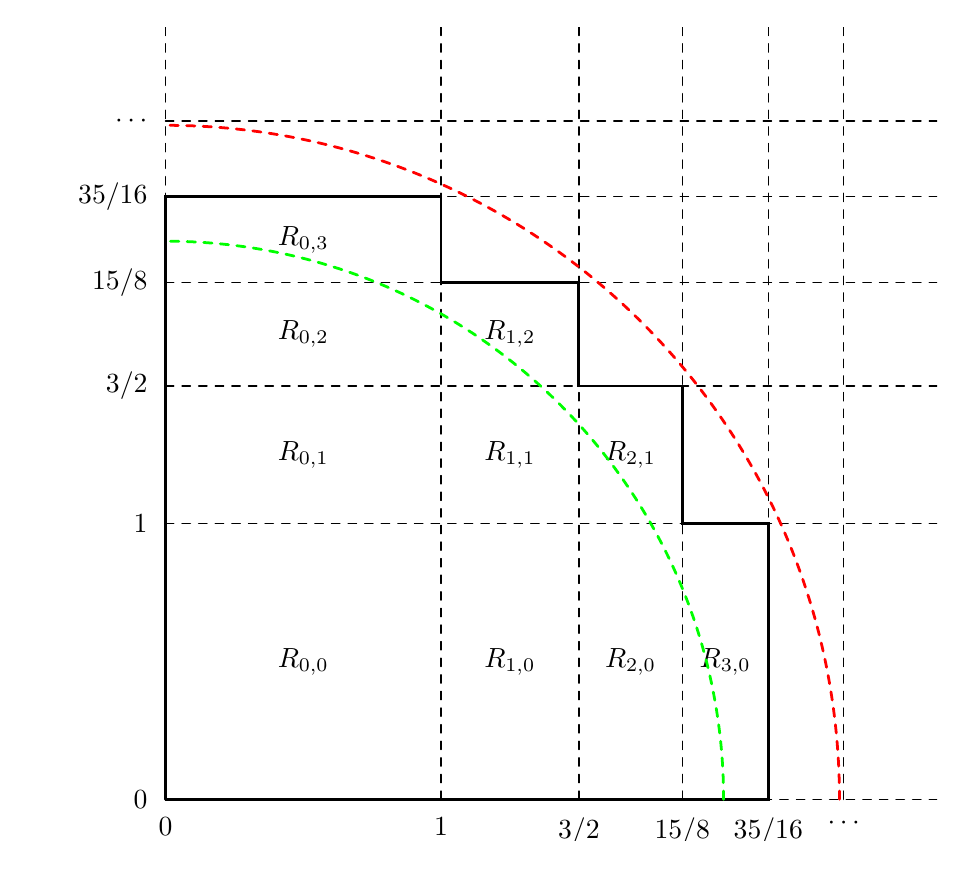
\begin{tikzpicture}[cap=round,scale=3.5]
\def\a{0}
\def\b{1}
\def\c{1.5}
\def\d{1.875}
\def\e{2.1875}
\def\f{2.4609375}
\def\ab{0.5}
\def\bc{1.25}
\def\cd{1.6875}
\def\de{2.03125}
\clip(-0.5,-0.15) rectangle (2.8,2.8);
\def\mylist{0/0,1/1,1.5/{3/2},1.875/{15/8},2.1875/{35/16},2.4609375/{$\cdots$}}
\foreach \xx/\label in \mylist{
	\draw [line width=0.5pt,dashed] (0,\xx) -- (10,\xx);
	\draw [line width=0.5pt,dashed] (\xx,0) -- (\xx,10);
	\draw (\xx,-0.03) node[anchor=north] {\label};
	\draw (-0.03,\xx) node[anchor=east] {\label};
}
\draw [line width=1pt] (\a,\a) -- (\a,\e) -- (\b,\e) -- (\b,\d) -- (\c,\d) -- (\c,\c) -- (\d,\c) -- (\d,\b) -- (\e,\b) -- (\e,\a) -- (\a,\a) ;
\draw (\ab,\ab) node {$R_{0,0}$};
\draw (\ab,\bc) node {$R_{0,1}$};
\draw (\ab,\cd) node {$R_{0,2}$};
\draw (\ab,\de) node {$R_{0,3}$};
\draw (\bc,\ab) node {$R_{1,0}$};
\draw (\bc,\bc) node {$R_{1,1}$};
\draw (\bc,\cd) node {$R_{1,2}$};
\draw (\cd,\ab) node {$R_{2,0}$};
\draw (\cd,\bc) node {$R_{2,1}$};
\draw (\de,\ab) node {$R_{3,0}$};
\def\xx{2.4457}
\def\yy{2.0252}
\draw[dashed,red,line width=1pt] (\xx,0) arc [start angle=0, end angle=90, radius=\xx];
\draw[dashed,green,line width=1pt] (\yy,0) arc [start angle=0, end angle=90, radius=\yy];
\end{tikzpicture}
\end{figure*}

多边形 $P_n $ 往外凸的点是集合 $\{ (s_i, s_j)\ |\ \ i+j=n+1,\ 1\le i,j \le n \}$. 这些点到原点的距离是 $ \sqrt{s_i^2+s_j^2} $. 根据前面推出的 $ s_i $ 与 $ o_n $ 的大小关系有
\[ \sqrt{s_i^2+s_j^2} \le \sqrt{\frac{2i+2j}{o_n}} = \sqrt{\frac{2(n+1)}{o_n}} .\]

类似的, 这个多边形向内凹的点是集合  $\{ (s_k, s_l)\ |\ \ k+l=n,\ 0\le k,l \le n \}$. 根据前面推出的 $ s_i $ 与 $ e_n $ 的大小关系有
\[ \sqrt{s_k^2+s_l^2} \ge \sqrt{\frac{2k+2l-2}{e_n}} = \sqrt{\frac{2(n-1)}{e_n}} .\]

也就是说, 多边形 $ P_n $ 的边被夹在半径为 $ \sqrt{2(n-1)/e_n} $ 和 $ \sqrt{2(n+1)/o_n} $ 的两个四分之一圆之间. 上面的图中也画出了这两个圆. 于是他们的面积满足关系
\[ \pi\cdot\frac{n-1}{2e_n} \le n \le \pi\cdot\frac{n+1}{2o_n} ,\]
所以 \[ \frac{(n-1)\pi}{2n} \le e_n < o_n \le \frac{(n+1)\pi}{2n} .\]
当 $ n  \rightarrow  \infty $ 时, 不等式两边都是 $ \pi/2 $, 而 $ e_n $ 和 $ o_n $ 也都是 Wallis 乘积. 命题得证.

\newpage
%------------------------------------------------------------------------------%
\section{欧拉的奇迹}
本小节参考 William Dunham 所著的 "Euler's Miracle" 一文. 该文分析了一种交错的调和级数.
虽然调和级数是发散的, 欧拉改变了调和级数的某些项的符号, 得到了收敛的结果, 并且收敛值正好是 $ \pi $.

\subsection{欧拉交错级数}

这里讨论的级数定义如下:
\begin{align*}
E &= 1 + \frac{1}{2} + \frac{1}{3} + \frac{1}{4} - \frac{1}{5} + \frac{1}{6} + \frac{1}{7} + \frac{1}{8} + \frac{1}{9} - \frac{1}{10} \\ 
& + \frac{1}{11} + \frac{1}{12} - \frac{1}{13} + \frac{1}{14} - \frac{1}{15} + \frac{1}{16} - \frac{1}{17} + \frac{1}{18} + \frac{1}{19} - \frac{1}{20} \\
& + \frac{1}{21} + \frac{1}{22} + \frac{1}{23} + \frac{1}{24} + \frac{1}{25} - \frac{1}{26} + \frac{1}{27} + \frac{1}{28} - \frac{1}{29} - \frac{1}{30} \\
& + \frac{1}{31} + \frac{1}{32} + \frac{1}{33} - \frac{1}{34} - \frac{1}{35} + \cdots
\end{align*}

改变符号的规则为: 对于任意正整数 $ n $, 如果 $n$ 含有奇数个形如 $ 4k + 1$ 的素因子(包含重复的), 那么 $\dfrac{1}{n} $ 的符号就是负的.

为了证明这个结论, 欧拉使用了 4 条已有的结论. 

\begin{enumerate}
\item Leibniz 级数: 
\[ 1-\frac{1}{3}+\frac{1}{5}-\frac{1}{7} + \cdots =\frac{\pi}{4} \]
\item 巴塞尔问题: 
\[ 1+\frac{1}{2^2}+\frac{1}{3^2}+\cdots = \frac{\pi^2}{6} \]
\item 几何级数的求和:
\[ 1 + a + a^2 + a^3 + \cdots = \frac{1}{1-a}, \quad -1 < a < 1 \]
\item 算术基本定理或正整数唯一分解定理: 任何一个大于1的自然数, 如果它不为质数,那么它可以唯一分解成有限个质数的乘积.
\end{enumerate}

\subsection{Leibniz 级数的乘积形式}

欧拉的证明过程是先将 Leibniz 级数公式与它自身的 $\dfrac{1}{3}$ 相加:
\begin{align*}
\frac{\pi}{4} &= 1-\frac{1}{3}+\frac{1}{5}-\frac{1}{7} +\frac{1}{9} - \frac{1}{11} + \frac{1}{13} - \frac{1}{15} + \frac{1}{17} - \frac{1}{19} + \frac{1}{21} - \frac{1}{23} +\cdots \\
\frac{1}{3}\cdot\frac{\pi}{4} &= \frac{1}{3}-\frac{1}{9}+\frac{1}{15}-\frac{1}{21}+\cdots \\
\frac{\pi}{4}(1+\frac{1}{3})&=1+\frac{1}{5}-\frac{1}{7}-\frac{1}{11}+\frac{1}{13}+\frac{1}{17}-\frac{1}{19}-\frac{1}{23}+\cdots
\end{align*}

最后一个式子里, 分母为 3 的倍数的项被消去了. 接着再减去上面最后一个等式的 $\dfrac{1}{5}$, 得到:
\begin{align*}
\frac{\pi}{4}(1+\frac{1}{3})&=1+\frac{1}{5}-\frac{1}{7}-\frac{1}{11}+\frac{1}{13}+\frac{1}{17}-\frac{1}{19}-\frac{1}{23}+\cdots\\
\frac{1}{5}\cdot\frac{\pi}{4}(1+\frac{1}{3}) &= \frac{1}{5} + \frac{1}{25} - \frac{1}{35} - \cdots \\
\frac{\pi}{4}(1+\frac{1}{3})(1-\frac{1}{5})&=1-\frac{1}{7}-\frac{1}{11}+\frac{1}{13}+\frac{1}{17}-\frac{1}{19}-\frac{1}{23}+\cdots
\end{align*}

这里, 分母是 3 和 5 的倍数的项都没了. 如此, 再加上上面式子的 $\dfrac{1}{7}$:
\[  
\frac{\pi}{4}(1+\frac{1}{3})(1-\frac{1}{5})(1+\frac{1}{7}) = 1- \frac{1}{11}+\frac{1}{13}+\frac{1}{17}-\frac{1}{19} - \frac{1}{23} + \cdots
\]

以此类推, 每一步等式右边开头都是 $ 1\pm\dfrac{1}{p} $ 的形式, 其中 $ p $ 是一个质数. 无限重复下去, 根据 $\dfrac{1}{p}$ 在 Leibniz 级数中的正负号决定下一步乘上的是 $(1+\dfrac{1}{p})$ 还是 $(1-\dfrac{1}{p})$. Leibniz 级数中的正负号规律很容易看出来, $\dfrac{1}{4k+1}$ 是加号, $\dfrac{1}{4k+3}$ 是减号. 于是, 将上面的过程无限重复, 将得到: 
\[
\frac{\pi}{4}(1+\frac{1}{3})(1-\frac{1}{5})(1+\frac{1}{7})(1+\frac{1}{11})(1-\frac{1}{13})(1-\frac{1}{17})(1+\frac{1}{19}) \cdots = 1
\] 
或者写成:
\[
(1+\frac{1}{3})(1-\frac{1}{5})(1+\frac{1}{7})(1+\frac{1}{11})(1-\frac{1}{13})(1-\frac{1}{17})(1+\frac{1}{19}) \cdots = \frac{4}{\pi}
\]

如此就把求和形式的 Leibniz 级数转成了乘积形式.

\subsection{巴塞尔问题的乘积形式}
考虑下面的分式, 分母中各项里的分数的分母包含了所有质数:
\[
Q = \frac{1}{(1+\frac{1}{2})(1-\frac{1}{2})(1+\frac{1}{3})(1-\frac{1}{3})(1+\frac{1}{5})(1-\frac{1}{5})(1+\frac{1}{7})(1-\frac{1}{7})(1+\frac{1}{11})(1-\frac{1}{11})\cdots}
\]

欧拉将它的相邻项两两结合, 并使用几何级数展开:
\begin{align*}
Q &= \frac{1}{1-\frac{1}{4}}\cdot\frac{1}{1-\frac{1}{9}}\cdot\frac{1}{1-\frac{1}{25}}\cdot\frac{1}{1-\frac{1}{49}}\cdot\frac{1}{1-\frac{1}{121}}\cdot\frac{1}{1-\frac{1}{169}}\cdot\cdots \\
 &= \left(1+\frac{1}{4}+\frac{1}{4^2}+\cdots\right)\left(1+\frac{1}{9}+\frac{1}{9^2}+\cdots\right)\left(1+\frac{1}{25}+\cdots\right)\left(1+\frac{1}{49}+\cdots\right)\cdots
\end{align*}

可以断言, 巴塞尔问题中的任意一项 $ \dfrac{1}{N^2}$会在这个乘积中出现且仅出现一次. 这是因为 $ N $ 可以被唯一地表示成质数的乘积: $ N = \prod p_i^{k_i} $, 其中 $ p_i $ 是第 $ i $ 个质数, $ k_i $ 是自然数.
则 $ N^2 = \prod (p_i^2)^{k_i} $. 每个 $ N $ 对应一组 $\{k_i\}$ 的序列, 且该序列非零项个数是有限的. 而这样的序列一一对应了上面乘积展开式中的一项. 于是
\[Q = 1 + \frac{1}{4} + \frac{1}{9} + \frac{1}{16} + \cdots = \frac{\pi^2}{6} .\]

或者写成
\[(1+\frac{1}{2})(1-\frac{1}{2})(1+\frac{1}{3})(1-\frac{1}{3})(1+\frac{1}{5})(1-\frac{1}{5})(1+\frac{1}{7})(1-\frac{1}{7})\cdots= \frac{1}{Q} = \frac{6}{\pi^2}\]

左边是 $(1\pm\frac{1}{p})$ 形式的乘积, $p$ 为质数.

\subsection{证明结论}

得到了前述的 Leibniz 级数和巴塞尔问题的乘积形式后, 将二者相除, 在乘以 $ \dfrac{3}{2} $, 得到
\begin{align*}
 \pi &= \frac{3}{2}\left[\frac{4/\pi}{6/\pi^2}\right] \\
&=  \frac{3}{2}\left[\frac{(1+\frac{1}{3})(1-\frac{1}{5})(1+\frac{1}{7})(1+\frac{1}{11})(1-\frac{1}{13})(1-\frac{1}{17})(1+\frac{1}{19})\cdots}{(1+\frac{1}{2})(1-\frac{1}{2})(1+\frac{1}{3})(1-\frac{1}{3})(1+\frac{1}{5})(1-\frac{1}{5})(1+\frac{1}{7})(1-\frac{1}{7})\cdots}\right] \\
&= \frac{1}{1-\frac{1}{2}}\cdot\frac{1}{1-\frac{1}{3}}\cdot\frac{1}{1+\frac{1}{5}}\cdot\frac{1}{1-\frac{1}{7}}\cdot\frac{1}{1-\frac{1}{11}}\cdot\frac{1}{1+\frac{1}{13}}\cdot\frac{1}{1+\frac{1}{17}}\cdot\frac{1}{1-\frac{1}{19}}\cdots
\end{align*}
可以发现, 最后的式子中, 对于奇素数 $ p $, 如果 $p$ 是 $4k+1$ 的形式, 则对应 $\left(1+\dfrac{1}{p}\right)^{-1}$ 的项; 如果 $p$ 是 $4k+3$ 的形式, 则对应 $\left(1-\dfrac{1}{p}\right)^{-1}$ 的项.

继续应用几何级数展开, 得到
\begin{align*}
\pi = & \left(1+\frac{1}{2}+\frac{1}{2^2}+\cdots\right)\times\left(1+\frac{1}{3}+\frac{1}{3^2}+\cdots\right)\times\left(1-\frac{1}{5}+\frac{1}{5^2}-\cdots\right)\times\\
& \left(1+\frac{1}{7}+\frac{1}{7^2}+\cdots\right)\times\left(1+\frac{1}{11}+\frac{1}{11^2}+\cdots\right)\times\left(1-\frac{1}{13}+\frac{1}{13^2}-\cdots\right)\times\cdots
\end{align*}

这些乘积中的每一个级数, 有些全是加号, 有些是加减号交错的. 将乘积展开就能得到调和级数的每一项, 并且是一一对应的. 如果分母恰有奇数个 $4k+1$ 形式的素因数, 在欧拉交错级数中就是减号. 

\newpage
%------------------------------------------------------------------------------%
\section{二项式定理的推广}
\subsection{杨辉三角的扩展}
二项式定理: \[(1+x)^n = \sum_{k=0}^{n}{C_n^k}x^k \].
其中组合数 $ C_n^k $ 使用下面的方式计算: \[ C_n^k = \frac{n!}{k!(n-k)!} = \frac{n\cdot(n-1)\cdots 2\cdot 1}{k!\cdot(n-k)(n-k-1)\cdots 2\cdot 1} = \frac{n\cdot(n-1)\cdots (n-k+1)}{k!}\]
因为 $ k $ 是自然数, 当 $ n >= 0 $ 时, 对于 $ k \ge n $, 分子中总是会存在 $ (n-n) $ 的一项. 所以展开式只有有限项.

如果 $ n < 0 $ 又如何? 多项式展开系数可以通过所谓的杨辉三角递推地求出来, 杨辉三角一般写成下面的样子:
%\begin{figure*}[htpb]
\begin{center}
\begin{tabular}{>{$n=}l<{$\hspace{12pt}}*{13}{c}}
0 &1&&&&&&&&&&&&\\
1 &1&&1&&&&&&&&&&\\
2 &1&&2&&1&&&&&&&&\\
3 &1&&3&&3&&1&&&&&&\\
4 &1&&4&&6&&4&&1&&&&\\
5 &1&&5&&10&&10&&5&&1&&\\
6 &1&&6&&15&&20&&15&&6&&1
\end{tabular}
\end{center}
%\end{figure*}
对于任意 $ n $, 
\[ (1+x)^{n+1} = (1+x)(1+x)^n = \sum_{k=0}^{n}{C_n^k}x^k + x\sum_{k=0}^{n}{C_n^k}x^k .\]
容易得到 $ (1+x)^{n+1} $ 的 $ k $ 次幂系数是 $ (1+x)^n $ 的 $ k $ 次幂 与 $ k - 1 $ 次幂的系数之和, 或 $ C_{n+1}^k = C_n^{k-1} + C_n^k $. 这也就是杨辉三角相邻两层之间的递推关系.

注意这个关系的推出并没有限制 $ n \ge 0 $. 我们可以尝试对杨辉三角往上做扩充. 把每行的空位填上 $ 0 $, 并且上下两层之间仍然满足递推关系:
\begin{center}
\begin{tabular}{>{$n=}l<{$\hspace{12pt}}*{13}{c}}
-4&1&&-4&&10&&-20&&35&&-56&&84\\
-3&1&&-3&&6&&-10&&15&&-21&&28\\
-2&1&&-2&&3&&-4&&5&&-6&&7\\
-1&1&&-1&&1&&-1&&1&&-1&&1\\
0 &1&&0&&0&&0&&0&&0&&0\\
1 &1&&1&&0&&0&&0&&0&&0\\
2 &1&&2&&1&&0&&0&&0&&0\\
3 &1&&3&&3&&1&&0&&0&&0\\
4 &1&&4&&6&&4&&1&&0&&0\\
5 &1&&5&&10&&10&&5&&1&&0\\
6 &1&&6&&15&&20&&15&&6&&1
\end{tabular}
\end{center}
于是有下面的级数展开, 可以用泰勒级数验证其正确性:
\begin{align*}
(1+x)^{-1} &= 1-x+x^2-x^3+x^4-x^5+\cdots \\
(1+x)^{-2} &= 1-2x+3x^2-4x^3+5x^4-6x^5+\cdots \\
\cdots
\end{align*}

\subsection{分数次幂}
当 $ n $ 不再是整数时, 二项式定理仍然成立. 可以用泰勒级数证明. 例如, 
\[ (1+x)^{\frac{1}{2}} = 1 + \frac{1}{2}x + \frac{1}{2!}\cdot\frac{1}{2}\cdot(\frac{1}{2}-1)x^2+ \frac{1}{3!}\cdot\frac{1}{2}\cdot(\frac{1}{2}-1)\cdot(\frac{1}{2}-2)x^3+\cdots \]

杨辉三角的递推关系也成立. 这意味着我们可以从 $ (1+x) $ 的 $ n $ 次幂展开系数推出 $ n + 1 $, $ n - 1 $, $ n + 2 $, $ n - 2 $ 等等次幂的展开系数. 

下面介绍的两个应用都巧妙的利用了 $ (1+x) ^\frac{1}{2} $ 的多项式展开.

\subsection{速算开方}
以计算 $ \sqrt{3} $ 为例, 取 $ x = -\dfrac{1}{4} $, 有
\begin{align*}
\sqrt{3} &= \sqrt{4(1-\frac{1}{4})} \\
			&= 2(1-\frac{1}{4})^\frac{1}{2}\\
			&= 2\left( 1+\frac{1}{2}(-\frac{1}{4}) + \frac{1}{2!}\frac{1}{2}(-\frac{1}{2})(-\frac{1}{4})^2 + \cdots \right)
\end{align*}

\subsection{牛顿的速算 $\pi$ 的算法}
单位圆的方程为 $ x^2 + y^2 = 1 $, 考虑用积分求第一象限的1/4圆 $ y = \sqrt{1-x^2} $ 的面积:
\begin{align*}
\frac{\pi}{4} &= \int_0^1{(1-x^2)^\frac{1}{2} dx} \\
				&=\int_0^1\left[1-\frac{1}{2}x^2-\frac{1}{8}x^4-\frac{1}{16}x^6-\frac{5}{128}x^8-\cdots\right] dx \\
\pi &= 4\left[x - \frac{1}{6}x^3 - \frac{1}{40}x^5 - \frac{1}{112}x^7 - \frac{5}{1152}x^9 - \cdots \right]^1_0 \\
	&= 4\left[1-\frac{1}{6} - \frac{1}{40} - \frac{1}{112} - \frac{5}{1152} - \cdots \right]
\end{align*}
这样得出来的结果收敛速度不够快, 如果积分上限是 $ \frac{1}{2} $, 那么余项会以指数的速度缩小.
\begin{figure*}[htbp]
\centering
\definecolor{wrwrwr}{rgb}{0.3803921568627451,0.3803921568627451,0.3803921568627451}
\definecolor{rvwvcq}{rgb}{0.08235294117647059,0.396078431372549,0.7529411764705882}
\subfigure{
\begin{minipage}[b]{0.48\linewidth}
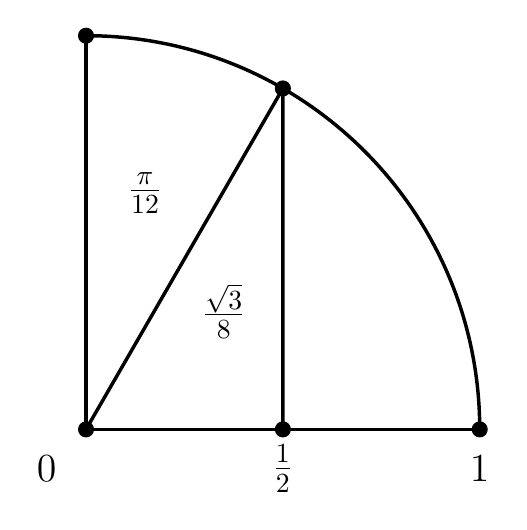
\begin{tikzpicture}[scale=5]
\coordinate[] (O) at (0.0,0.0);
\coordinate[] (A) at (1.0,0.0);
\coordinate[] (B) at (0.0,1.0);
\coordinate[] (C) at (0.5,0.866);
\coordinate[] (D) at (0.5,0.0);
\draw[line width=1.25pt] (A) -- (O) -- (B);
\draw[line width=1.25pt] (A) arc (0:90:1);
\draw[line width=1.25pt] (O) -- (C) -- (D);
\foreach \p in {O,A,B,C,D}
	\fill[fill=black,draw=black,thick] (\p) circle (0.5pt);
\draw[font=\Large] (-0.1, -0.1) node {$0$};
\draw[font=\Large] (1.0, -0.1) node {$1$};
\draw[font=\Large] (0.5, -0.1) node {$\frac{1}{2}$};
\draw[font=\Large] (0.15, 0.6) node {$\frac{\pi}{12}$};
\draw[font=\Large] (0.35, 0.3) node {$\frac{\sqrt{3}}{8}$};
\end{tikzpicture}
\end{minipage}}
\subfigure{
\begin{minipage}[b]{0.48\linewidth}
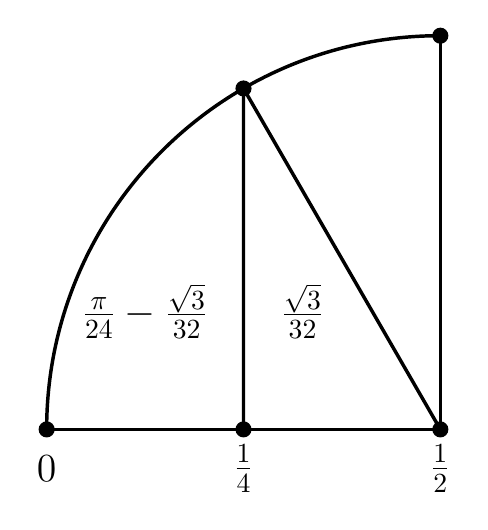
\begin{tikzpicture}[scale=5]
\coordinate[] (O) at (0.0,0.0);
\coordinate[] (A) at (1.0,0.0);
\coordinate[] (B) at (1.0,1.0);
\coordinate[] (C) at (0.5,0.866);
\coordinate[] (D) at (0.5,0.0);
\draw[line width=1.25pt] (O) -- (A) -- (B);
\draw[line width=1.25pt] (B) arc (90:180:1);
\draw[line width=1.25pt] (A) -- (C) -- (D);
\foreach \p in {O,A,B,C,D}
	\fill[fill=black,draw=black,thick] (\p) circle (0.5pt);
\draw[font=\Large] (-0.0, -0.1) node {$0$};
\draw[font=\Large] (1.0, -0.1) node {$\frac{1}{2}$};
\draw[font=\Large] (0.5, -0.1) node {$\frac{1}{4}$};
\draw[font=\Large] (0.25, 0.3) node {$\frac{\pi}{24}- \frac{\sqrt{3}}{32}$ };
\draw[font=\Large] (0.65, 0.3) node {$\frac{\sqrt{3}}{32}$};
\end{tikzpicture}
\end{minipage}}
\end{figure*}

如图所示, 积分区间取 $ [0, \frac{1}{2} ] $ 对应的区域可以划分成一个扇形和一个直角三角形, 扇形面积是 $ \pi/12 $, 三角形面积是 $ \sqrt{3}/8 $. 所以:
\[
\frac{\pi}{12}+\frac{\sqrt{3}}{8} = \int_0^\frac{1}{2}{(1-x^2)^\frac{1}{2} dx} 
\]
\[
\pi = 12\left[ -\frac{\sqrt{3}}{8} + \frac{1}{2}-\frac{1}{6}(\frac{1}{2})^3-\frac{1}{40}(\frac{1}{2})^5 - \frac{1}{112}(\frac{1}{2})^7 - \frac{5}{1152}(\frac{1}{2})^9 - \cdots \right]
\]

另一种减小积分上限的方法是考虑圆的方程是 $ x^2 - x + y^2 = 0 $, 它的圆心在 $ (\dfrac{1}{2}, 0) $, 半径为 $ \dfrac{1}{2} $. 积分区间是 $ [0,\frac{1}{4} ]$, 被积函数是 $ y = \sqrt(x - x^2) $, 面积关系为:
\begin{align*}
\frac{\pi}{24} - \frac{\sqrt{3}}{32} &= \int_0^\frac{1}{4}{x^\frac{1}{2}(1-x)^\frac{1}{2} dx} \\
		&= \int_0^\frac{1}{4}{ x^\frac{1}{2}\left[ 1-\frac{1}{2}x - \frac{1}{8}x^2-\frac{1}{16}x^3-\frac{5}{128}x^4-\cdots \right] dx} \\
		&= \int_0^\frac{1}{4}{ \left[ x^\frac{1}{2}-\frac{1}{2}x^\frac{3}{2}-\frac{1}{8}x^\frac{5}{2}-\frac{1}{16}x^\frac{7}{2}-\frac{5}{128}x^\frac{9}{2}-\cdots \right] dx} \\
		&= \left[ \frac{2}{3}x^\frac{3}{2} - \frac{1}{2}\cdot\frac{2}{5}x^\frac{5}{2}-\frac{1}{8}\cdot\frac{2}{7}x^\frac{7}{2}-\frac{1}{16}\cdot\frac{2}{9}x^\frac{9}{2}-\frac{5}{128}\cdot\frac{2}{11}x^\frac{11}{2} - \cdots \right]_0^\frac{1}{4} \\
\pi &= \frac{3\sqrt{3}}{4}+24\left(\frac{1}{12}-\frac{1}{5\cdot 2^5}-\frac{1}{28\cdot 2^7} -\frac{1}{72\cdot 2^9} - \frac{5}{704\cdot 2^{11}} -\cdots \right) 
\end{align*}


\newpage
%------------------------------------------------------------------------------%
\section{阿基米德如何计算球的表面积}

核心思想在于将球的表面与一个正好包住球的圆柱体侧面建立联系, 假设球的半径为 $R$, 则圆柱的底面半径为 $R$, 高为 $2R$, 侧面积正好是 $2\pi R\cdot 2R=4\pi R^2$, 如下图所示:
\begin{figure}[htbp]
\centering

\begin{minipage}[t]{0.35\linewidth}
\centering
\begin{tikzpicture}[]
  \coordinate (O) at (0,0);
\coordinate (1) at (0,1.41);
\coordinate (2) at (0,2);
\coordinate (3) at (1.41,1.41);
  % ball background color
  \shade[ball color = white, opacity = 0.2] (0,0) circle [radius = 2cm];
  % ball
  \draw (O) circle [radius=2cm];
  % label of ball center point
  % \filldraw (O) circle (1pt) node[below] {$O$};
  % radius
%  \draw[densely dashed] (O) -- (-1.33,1.33);
  \draw[densely dashed] (1.33,1.33) to [edge label = $R$] (O);
  % cut of ball surface
  %\draw[red] (-1.35,1.47) arc [start angle = 140, end angle = 40, x radius = 17.6mm, y radius = 14.75mm];	% top
  \draw[red, densely dashed] (-1.36,1.46) arc [start angle = 170, end angle = 10, x radius = 13.8mm, y radius = 3.6mm];
  \draw[red] (-1.29,1.52) arc [start angle=-200, end angle = 20, x radius = 13.75mm, y radius = 3.15mm];
  \draw[red] (-1.45,1.35) arc [start angle=-200, end angle = 20, x radius = 15.5mm, y radius = 3.5mm];
\filldraw (1) circle (1pt);
 \draw[green] (0,2) arc [start angle=90, end angle =-90, x radius = -16.5mm, y radius = 20mm];
 \draw[green] (0,2) arc [start angle=90, end angle =-90, x radius = -14.5mm, y radius = 20mm];
\draw[densely dashed] (1) to (-1.3, 1.3);
\draw[densely dashed] (1) to (-1.15, 1.22);
\filldraw (1) circle (1pt);
\draw[densely dashed] (1) to (3);
\draw[densely dashed] (0,-2) -- (2);
\draw
    (0,2) coordinate (a)
    (0,0) coordinate (b)
    (1.41,1.41) coordinate (c)
    pic["$\phi$", draw,<-, angle eccentricity=1.5, angle radius=0.5cm]
    {angle=c--b--a};
%cylinder
\draw[] (-2, -2) -- (-2,2) -- (2,2) -- (2,-2);
\draw[densely dashed] (2, -2) -- (-2,-2);
\draw[densely dashed] (-1.98,-2.05) arc [start angle = 180, end angle = 0, x radius = 20.0mm, y radius = 5.0mm];
\draw[] (-1.98,-2.05) arc [start angle=-180, end angle = 0, x radius = 20.0mm, y radius = 5.0mm];
\draw[densely dashed] (-1.98,2.05) arc [start angle = 180, end angle = 0, x radius = 20.0mm, y radius = 5.0mm];
\draw[] (-1.98,2.05) arc [start angle=-180, end angle = 0, x radius = 20.0mm, y radius = 5.0mm];
\filldraw (0,-2) circle (1pt);
\filldraw (0,2) circle (1pt);
\end{tikzpicture}
\end{minipage}
\begin{minipage}[t]{0.59\linewidth}
\centering
\begin{tikzpicture}[]
\draw[] (-4,2) -- (4,2) -- (4,-2);
\draw[] (-4,-2) to [edge label = $2 R$] (-4, 2);
\draw[] (4,-2) to [edge label = $2\pi R$] (-4, -2);
\draw[red] (-4,1.41) -- (4,1.41);
\draw[red] (-4,1.2) -- (4,1.2);
\draw[green] (-2.2,-2) to  (-2.2, 2);
\draw[green] (-2.0,-2) to  (-2.0, 2);
\end{tikzpicture}
\end{minipage}
\end{figure}

用球面坐标系, $(\theta, \phi)$ 表示经纬度, $\theta \in [0, 2\pi), \phi \in [0,\pi]$, 且 $\phi=0$ 表示北极点. 考虑点 $(\theta, \phi)$ 处的面积微元, 在经线方向上是 $R\sin\phi\ \mathrm{d}\theta$, 在纬线方向上是 $R\ \mathrm{d}\phi$, 于是微元为 $\mathrm{d}s = R^2\sin\phi\ \mathrm{d}\theta\ \mathrm{d}\phi$.

再假想有一个光源, 能在 $z$ 轴上各处向四面八方发射光线, 考虑上述面积微元在圆柱侧面的投影. 
经线方向是将半径为 $r=R\sin\phi$, 角度为 $\mathrm{d}\theta$ 的一段圆弧投影到半径为 $R$ 的圆弧上, 所以长度为 $R\ \mathrm{d}\theta$. 
纬线方向是将半径为 $R$, 角度为 $\mathrm{d}\phi$ 的一段圆弧投影到 $z$ 轴上, 而这段圆弧的法向与 $z$ 轴的夹角为 $\phi$, 于是投影的长度为 $R\ \mathrm{d}\phi\cdot\sin\phi$. 
两个方向上乘起来得到投影之后的面积微元仍然是 $\mathrm{d}S = R^2\sin\phi\ \mathrm{d}\theta\ \mathrm{d}\phi$. 说明投影保持了面积大小不变, 所以圆柱侧面积和球表面积相等.

\begin{figure}[htbp]
\centering
\begin{minipage}[t]{0.48\linewidth}
\centering
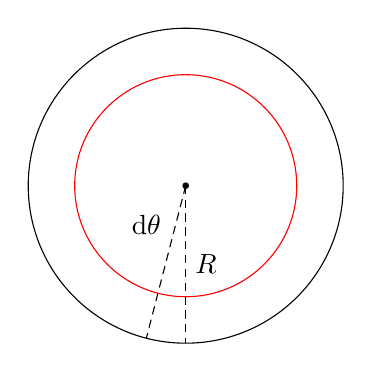
\begin{tikzpicture}[]
  \coordinate (O) at (0,0);
\coordinate (1) at (0,1.41);
\coordinate (2) at (0,2);
\coordinate (3) at (1.41,1.41);
  \draw (O) circle [radius=2cm];
\filldraw (0,0) circle (1pt);
\draw[densely dashed] (0,0) to [edge label = $R$] (0,-2);
\draw[densely dashed] (0,0) to (-0.5,-1.936);
%\draw[red] (0, -1.41) arc [start angle = -90, end angle = -105, radius = 1.41];
\draw[red]  (O) circle [radius=1.41cm];
\draw (-0.5,-0.5) node {$\mathrm{d}\theta$};
\end{tikzpicture}
\end{minipage}
\begin{minipage}[t]{0.48\linewidth}
\centering
\begin{tikzpicture}[]
  \coordinate (O) at (0,0);
\coordinate (1) at (0,1.41);
\coordinate (2) at (0,2);
\coordinate (3) at (1.41,1.41);
  \draw[green] (O) circle [radius=2cm];
\filldraw (0,0) circle (1pt);
\draw[densely dashed] (0,0) to [edge label = $R$] (0,2);
\draw[densely dashed] (0,0) to (1,1.732);
\draw[densely dashed] (0,0) to (1.2,1.6);
\draw
    (0,2) coordinate (a)
    (0,0) coordinate (b)
    (1.0,1.732) coordinate (c)
    pic["$\phi$", draw,<-, angle eccentricity=1.5, angle radius=0.5cm]
    {angle=c--b--a};
\draw (2,-2) to (2,2);
\draw [densely dashed](0,1.732) to (2,1.732);
\draw [densely dashed](0,1.6) to (2,1.6);
\end{tikzpicture}
\end{minipage}
\end{figure}

上图示意了投影的过程. 左边是纬线的投影, 从 $z+$ 方向俯视, 红线代表纬线. 一段纬线上的圆弧, 投射到外层圆柱上之后, 长度拉伸了 $\sin\phi$ 倍. 上图右边是经线的投影, 视线垂直于经线和 $z$ 轴所在平面. 经线上的一小段圆弧的切线方向与 $xy$ 平面夹角是 $\phi$, 投影到 $z$ 轴或圆柱侧面上时, 缩短的比例为 $\sin\phi$. 纬线上的拉伸和经线上的缩短正好抵消了.

\newpage
%------------------------------------------------------------------------------%
\section{Fibonacci 数列}

一般 Fibonacci 数列定义如下: $x_0 = 0, x_1 = 1, x_{n+1} = x_{n} + x_{n-1} $.

\subsection{通项公式: 初等解法}

我们尝试将递推关系凑出下面的形式: 
\[ x_{n+1} + ax_n = b(x_n+ax_{n-1}) .\]
从而可以令 $ y_n = x_{n+1} + ax_n $, 然后求出 $ y_n $, 进而求出 $ x_n $.

比较系数可以得到: $ b - a = 1 $, $ ab = 1 $.于是可以解出 $ a = \dfrac{\sqrt{5}-1}{2}$, $ b = \dfrac{\sqrt{5}+1}{2}$.
进一步, $y_0 = x_1+ax_0 = 1 $, $ y_n = b^n $.
\begin{align*} 
x_{n+1}+ax_n &= b^n \\
ax_n+a^2x_{n-1} &= ab^{n-1} \\
\cdots & \\
a^{n-1}x_2 + a^{n}x_1 &= a^{n-1}b \\
a^{n}x_1 + a^{n+1}x_0 &= a^nb^{0}
\end{align*}

错位相减得 $ x_{n+1} = b^n - ab^{n-1} + a^2b^{n-2} - \cdots + (-1)^na^n $. 这是一个等比数列之和, 注意到 $ a $ 和 $ b $ 互为倒数, 公比是 $ -ab^{-1}=-a^2 $, 这个的和其实就是:
\[ x_{n+1} = \frac{b^n-(-a)^n(-a^2)}{1-(-a^2)} = \frac{b^{n+1}-(-a)^{n+1}}{b+a} = \frac{b^{n+1}-(-a)^{n+1}}{\sqrt{5}}.\]

所以通项公式是: 
\[ x_n = \frac{1}{\sqrt{5}}\left[ \left(\frac{\sqrt{5}+1}{2}\right)^n - \left(\frac{1-\sqrt{5}}{2}\right)^n \right] .\]

\subsection{通项公式: 矩阵解法}

Fibonacci 数列的递推关系可以写成矩阵的形式:
\[
\begin{bmatrix}
x_{n+1} \\
x_n 
\end{bmatrix} = 
\begin{bmatrix}
& 1 & 1 & \\
& 1 & 0 & 
\end{bmatrix}
\begin{bmatrix}
x_n \\
x_{n-1}
\end{bmatrix}
=F \begin{bmatrix}
x_n \\
x_{n-1}
\end{bmatrix}
=\cdots
=F^{n} \begin{bmatrix}
x_1 \\
x_0
\end{bmatrix}
\]
将矩阵 $ F $ 做对角化分解: $ F = P^{-1} \Lambda P $. 其中 
\[ \Lambda = \begin{bmatrix} -a & 0 \\ 0 & b \end{bmatrix} , P = \frac{1}{\sqrt{5}}\begin{bmatrix} -1 & b \\ 1 & a \end{bmatrix}, P^{-1} = \begin{bmatrix} -a & b \\ 1 & 1 \end{bmatrix} .\]
则 
\begin{align*}
F^{n} &= P^{-1}\Lambda^{n} P \\
% &= \frac{1}{\sqrt{5}}\begin{bmatrix}
%-a & b \\ 1 & 1
%\end{bmatrix}
%\begin{bmatrix}
%(-a)^{n} & 0 \\ 0 & b^{n}
%\end{bmatrix}
%\begin{bmatrix}
%-1 & b \\ 1 & a
%\end{bmatrix} \\
 &= \frac{1}{\sqrt{5}}\begin{bmatrix}
b^{n+1} - (-a)^{n+1} & ab^{n+1}+b(-a)^{n+1} \\b^n - (-a)^n & ab^n+b(-a)^n 
\end{bmatrix} 
.\end{align*}
代入 $x_1$ 和 $ x_0$ 的值可以得到通项: $x_n = \dfrac{1}{\sqrt{5}}\left(b^n - (-a)^n\right)$.

\subsection {模的周期}
考虑 Fibonacci 数列关于整数 $m$ 的模, 下面的讨论均是在模 $m$ 的意义下进行. 

先研究相邻两项组成的二元组 $(x_{n+1},x_n)$ 模 $m$ 的余数. 这样的余数二元组最多有 $ m^2 $ 种可能, 所以一定会出现重复的. 不妨令 $(x_{k+1},x_k) \equiv (x_{k+p+1},x_{k+p}) $, 根据上面的矩阵形式的递推关系, 有:
\[
F^k
\begin{bmatrix}
x_{1} \\ x_0
\end{bmatrix}
\equiv  F^{k+p}
\begin{bmatrix}
x_{1} \\ x_0
\end{bmatrix}
\]
而矩阵 $ F $ 是可逆的, 我们把上面等式两边都乘以 $ F^{-k} $, 可知二元组 $(x_1,x_0)$ 经过 $ p $ 次以后又回到了 $(x_1,x_0)$. 

另一个结论是: 如果 $ m = x_p $, 则模 $ m $ 的循环周期是 $ p $. 例如, $ x_4 = 3 $, $ x_{4k} $ 都能被 $ 3 $ 整除.
\begin{table}[h!]
\centering
\begin{tabular}{ c c c c c c c c c c c c c c c c c }
\hline 
$n$ & 0 & 1 & 2 & 3 & 4 & 5 & 6 & 7 & 8 & 9 & 10 & 11 & 12 & 13 & 14 & $\cdots$\\
\hline 
$x_{n}$ & 0 & 1 & 1 & 2 & 3 & 5 & 8 & 13 & 21 & 34 & 55 & 89 & 144 & 233 & 377 & $\cdots$ \\
\hline 
\end{tabular}
\end{table}

这很容易证明. 显然, $ x_p \equiv 0 \pmod{x_p}$, 假设 $ x_{p+1} \equiv r \pmod{x_p} $, 后续序列分别是 $ r, r, 2r, 3r, 5r, \cdots $, 也就是将第一个周期内的序列乘以 $ r $ 再重复一遍, 这样到 $ x_{2p} $ 的时候余数又会回到 $ 0 $. 等等.

\subsection {Arnold 变换}

给一个 $ m\times m $ 的图像, 一次Arnold 变换是将 $ (x,y) $ 处的像素移动到 $ (2x+y, x+y) \bmod{m}$ 处. 重复若干次以后, 图像就会变得杂乱无章. 再继续进行变换, 图像会回到原来的样子. 由 Arnold 提出, 并且用例图片都是猫, 所以又被称为 "猫映射"(cat mapping).

记 $(x, y)$ 在经过 $n$ 次变换后的坐标是 $(x_n,y_n)$, 则
\[
\begin{bmatrix}
x_n \\ y_n
\end{bmatrix}
=\begin{bmatrix}
2 & 1 \\ 1 & 1
\end{bmatrix}^n
\begin{bmatrix}
x_0 \\ y_0
\end{bmatrix} = F^{2n} \begin{bmatrix}
x_0 \\ y_0
\end{bmatrix} \bmod{m}.
\]
由前面的分析可以知道 $F$ 经过循环周期会变成单位阵, 所以 Arnold 变换进行若干次也会得到原图像.

\subsection {1/89}
\begin{align*}
1/89 &= 0.01123595505617977528089887640449\cdots \\
	&= 0.0 \\
	 & + 0.01 \\
	&+ 0.001\\
	&+ 0.0002 \\
	&+ 0.00003\\
	&+ 0.000005\\
	&+ 0.0000008\\
	&+ 0.00000013\\
	&+ 0.000000021\\
	&+ 0.0000000034\\
	&+ 0.00000000055\\
	&+\cdots
\end{align*}

其实就是 $\dfrac{x_n}{10^n}$, 代入通项公式求和就是 $ 10 / 89 $.

\newpage
%------------------------------------------------------------------------------%
\section{Thebault problem}

任意一个四边形, 每边朝外作正方形, 连接相对两个正方形的中心, 得到的两组线段相互垂直且长度相等.
\begin{figure*}[htbp]
\centering
\definecolor{wrwrwr}{rgb}{0.3803921568627451,0.3803921568627451,0.3803921568627451}
\definecolor{rvwvcq}{rgb}{0.08235294117647059,0.396078431372549,0.7529411764705882}
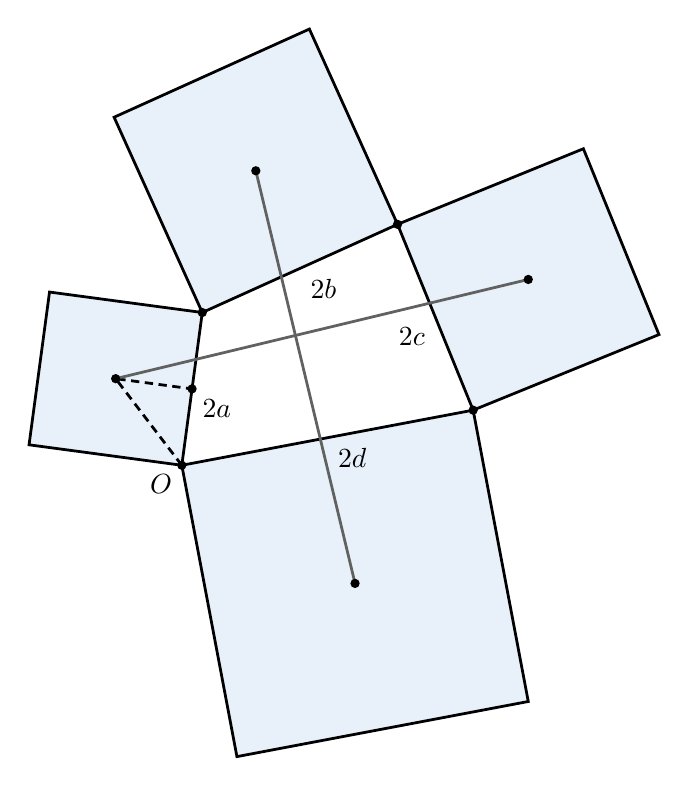
\begin{tikzpicture}[]
\coordinate[] (A) at (-1.88,1.68);
\coordinate[] (B) at (0.6,2.8);
\coordinate[] (C) at (1.56,0.44);
\coordinate[label=below left:$O$] (D) at (-2.14,-0.26);
\coordinate[] (AA) at (-1.2,3.48);
\coordinate[] (CC) at (0.06,-1.76);
\coordinate[] (BB) at (-2.98,0.84);
\coordinate[] (DD) at (2.26,2.1);
\coordinate[] (AAA) at (-2.01,0.71);

\draw[line width=1pt,fill=rvwvcq!10] (A) -- (-3.82,1.94) -- (-4.08,0) -- (D);
\draw[line width=1pt,fill=rvwvcq!10] (B) -- (-0.52,5.28) -- (-3,4.16) -- (A);
\draw[line width=1pt,fill=rvwvcq!10] (C) -- (3.92,1.4) -- (2.96,3.76) -- (B);
\draw[line width=1pt,fill=rvwvcq!10] (D) -- (-1.44,-3.96) -- (2.26,-3.26) -- (C);
% \draw[line width=1pt,arrows = {-Stealth[]}] (D) to [edge label' = $2a$] (A); 
\draw[line width=1pt] (D) to [edge label' = $2a$] (A); 
\draw[line width=1pt] (A) to [edge label' = $2b$] (B);
\draw[line width=1pt] (B) to [edge label' = $2c$] (C);
\draw[line width=1pt] (C) to [edge label = $2d$] (D);

%\draw[densely dashed,line width=1pt] (A) -- (AA)--(B);
%\draw[densely dashed,line width=1pt] (B) -- (DD)--(C);
%\draw[densely dashed,line width=1pt] (C) -- (CC)--(D);
\draw[densely dashed,line width=1pt] (D) -- (BB) -- (AAA);

\draw [line width=1pt,color=wrwrwr] (AA)-- (CC);
\draw [line width=1pt,color=wrwrwr] (BB)-- (DD);

\foreach \p in {AA,BB,CC,DD,A,B,C,D,AAA}
	\fill[fill=black,draw=black,thick] (\p) circle (1.25pt);
\end{tikzpicture}
\end{figure*}

\begin{proof}
假设沿顺时针方向, 四边形四条边对应的向量用复数表示分别是 $ 2a, 2b, 2c, 2d $, 假设 $ 2a $ 的起点为原点. 因为四边形是封闭的, 所以 $ a + b + c + d = 0 $. 

从原点出发, 走 $ a $, 再左转 $ 90\degree $ 后走相同的长度, 可以得到边 $ 2a $ 对应的正方形中心为 \[ P_1 = a + ae^{i\frac{\pi}{2}} = a(1+i). \]
其他正方形的中心分别为 
\begin{align*} 
P_2 &= 2a + b(1+i) \\ 
P_3 &= 2a + 2b + c(1+i) \\
P_4 &= 2a + 2b + 2c + d(1+i).
\end{align*}
连接相对两个正方形中心的线段对应的向量为以下两个复数:
\[ P_3 - P_1 = a + 2b + c + (c-a)i = b - d + (c-a)i, \]
\[ P_4 - P_2 = b + 2c + d + (d-b)i = c - a + (d-b)i. \]

容易发现 $ (P_3 - P_1) = (P_4 - P_2)i $, 所以它们相互垂直, 且长度相等.

\end{proof}

~

\noindent 另一种证明方法:

首先研究复平面上的平移和旋转变换, 用 $ T_v $ 表示平移一个向量 ( 或复数 ) $ v $ 的运算: $ T_v(z) = z + v $, 用 $ R_a^\theta $ 表示绕一点 $ a $ 旋转角度 $ \theta $. 其中绕原点的旋转可以写成 $ R_0^\theta(z) = e^{i\theta}z $.

一般的旋转等价于先把 $ a $ 平移到原点, 再绕原点旋转 $ \theta $, 最后把原点平移回 $ a $.
\[ R_a^\theta(z) = (T_a\circ R_0^\theta \circ T_a^{-1})(z) = e^{i\theta}(z-a)+a = e^{i\theta}z+k .\]
其中 $ k = a(1-e^{i\theta}) $. 也就是说, 任何旋转都可以表示成先绕原点做旋转, 再平移, 即: $ R_a^\theta = (T_k\circ R_0^\theta) $. 反过来也成立, 先绕原点旋转 $ \alpha $ 然后平移 $ v $ 的变换等价于绕某个点旋转同样的角度 $ \alpha $: 
\[ T_v \circ R_0^\alpha=R_c^\alpha ,\]
其中 $ c = v/(1-e^{i\alpha}) $. 类似的可以验证 $ R_0^\theta \circ T_v = R_p^\theta $.

考虑两个旋转的合成: 
\[ (R_b^\phi \circ R_a^\theta) (z) = e^{i(\theta+\phi)}z + v ,\]
其中 $ v = ae^{i\phi}(1-e^{i\theta})+b(1-e^{i\phi}) $.

一般而言, 若 $ \theta + \phi $ 不是 $ 2\pi $ 的整数倍, 则存在一个点 $ c $ 满足整个旋转等价于绕点 $ c $ 转 $ \theta + \phi $ 的角度:
\[ R_b^\phi \circ R_a^\theta = R_c^{(\theta+\phi)}, \]
$ c $ 的值可以由 $ a, b, \theta, \phi $ 表示, 这里略过.

若 $ \theta + \phi $ 是 $ 2\pi $ 的整数倍, 
\[ (R_b^\phi \circ R_a^\theta) (z) = z + (1-e^{i\phi})(b-a) ,\]
它其实是一个平移.

这个结论可以推广到多个旋转的合成, 如果一系列旋转变换的旋转角之和是 $ 2\pi $ 的整数倍, 则变换之后的结果等价于只进行平移.

\begin{figure*}[htbp]
\centering
\definecolor{wrwrwr}{rgb}{0.3803921568627451,0.3803921568627451,0.3803921568627451}
\definecolor{rvwvcq}{rgb}{0.08235294117647059,0.396078431372549,0.7529411764705882}
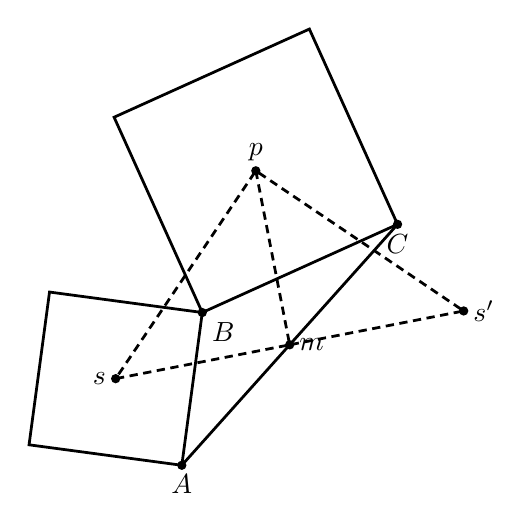
\begin{tikzpicture}[]
\coordinate[label=below right:$B$] (A) at (-1.88,1.68);
\coordinate[label=below:$C$] (B) at (0.6,2.8);
\coordinate[label=below:$A$] (D) at (-2.14,-0.26);
\coordinate[label=right:$m$] (M) at (-0.77,1.27);

\coordinate[label=above:$p$] (AA) at (-1.2,3.48);
\coordinate[label=left:$s$] (BB) at (-2.98,0.84);
\coordinate[label=right:$s'$] (SS) at (1.44, 1.7);
%\coordinate[] (DD) at (2.26,2.1);
% \coordinate[] (AAA) at (-2.01,0.71);

\draw[line width=1pt] (A) -- (-3.82,1.94) -- (-4.08,0) -- (D);
\draw[line width=1pt] (B) -- (-0.52,5.28) -- (-3,4.16) -- (A);
\draw[line width=1pt] (D) -- (A); 
\draw[line width=1pt] (A) -- (B);
%\draw[line width=1pt] (B) to [edge label' = $2c$] (C);
%\draw[line width=1pt] (C) to [edge label = $2d$] (D);

%\draw[densely dashed,line width=1pt] (A) -- (AA)--(B);
%\draw[densely dashed,line width=1pt] (B) -- (DD)--(C);
%\draw[densely dashed,line width=1pt] (C) -- (CC)--(D);
\draw[line width=1pt] (D) -- (B);
\draw[densely dashed,line width=1pt] (AA) -- (M) -- (BB) -- (AA) -- (SS) -- (M) ;

%\draw [line width=1pt,color=wrwrwr] (AA)-- (CC);
%\draw [line width=1pt,color=wrwrwr] (BB)-- (DD);

\foreach \p in {A,B,D,AA,BB,M,SS}
	\fill[fill=black,draw=black,thick] (\p) circle (1.25pt);
\end{tikzpicture}
\end{figure*}
现在回到原问题, 考虑四边形其中两条边 $ AB, BC $ 上的正方形, 正方形的中心为 $ s $ 和 $ p $, 对角线 $ AC $ 的中点为 $ m $, 再考虑三个旋转变换的复合 $ M = R_m^\pi \circ R_p^{(\pi/2)} \circ R_s^{(\pi/2)} $. 

因为三个旋转角度之和为 $ 2\pi $, 由之前的结论知道这其实是一个平移, 为了确定平移量, 考虑点 $ A $ 在这组变换下的结果, 先绕 $ s $ 转 $ 90\degree $ 变换到 $ B $ 点, 再绕 $ p $ 转 $ 90\degree $ 到达 $ C $ 点, 最后绕 $ m $ 转 $ 180\degree $ 回到 $ A $ 点. 

于是可以知道 $ M $ 其实是恒等变换. 从而 $ R_p^{(\pi/2)} \circ R_s^{(\pi/2)} = R_m^{-\pi} = R_m^\pi. $

定义点 $ s' $ 是 $ s $ 绕点 $ m $ 旋转 $ 180\degree $ 的结果: 
\[ s' = R_m^\pi(s) = R_p^{(\pi/2)} \circ R_s^{(\pi/2)}(s) = R_p^{(\pi/2)}(s).\] 
最后一个等号成立是因为 $ s $ 绕 $ s $ 旋转 $ 90\degree $ 仍然是自身.

这说明三角形 $ sps' $ 是等腰三角形, 且 $ \angle sps' $ 是直角. 进一步得到 $ sm $ 和 $ pm $ 垂直且等长.

\begin{figure*}[htbp]
\centering
\definecolor{wrwrwr}{rgb}{0.3803921568627451,0.3803921568627451,0.3803921568627451}
\definecolor{rvwvcq}{rgb}{0.08235294117647059,0.396078431372549,0.7529411764705882}
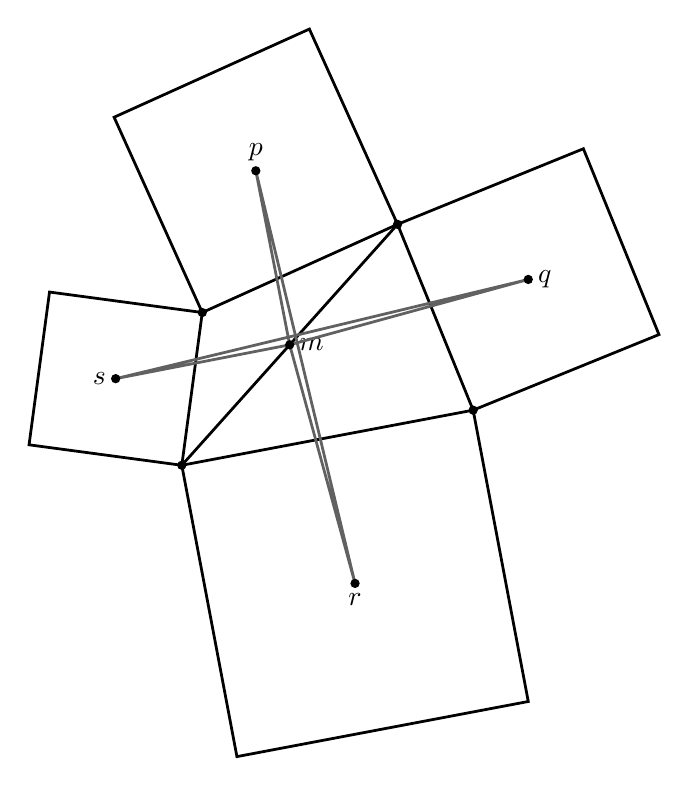
\begin{tikzpicture}[]
\coordinate[] (A) at (-1.88,1.68);
\coordinate[] (B) at (0.6,2.8);
\coordinate[] (C) at (1.56,0.44);
\coordinate[] (D) at (-2.14,-0.26);
\coordinate[label=above:$p$] (AA) at (-1.2,3.48);
\coordinate[label=below:$r$] (CC) at (0.06,-1.76);
\coordinate[label=left:$s$] (BB) at (-2.98,0.84);
\coordinate[label=right:$q$] (DD) at (2.26,2.1);
\coordinate[label=right:$m$] (M) at (-0.77,1.27);

\draw[line width=1pt] (A) -- (-3.82,1.94) -- (-4.08,0) -- (D);
\draw[line width=1pt] (B) -- (-0.52,5.28) -- (-3,4.16) -- (A);
\draw[line width=1pt] (C) -- (3.92,1.4) -- (2.96,3.76) -- (B);
\draw[line width=1pt] (D) -- (-1.44,-3.96) -- (2.26,-3.26) -- (C);
\draw[line width=1pt] (D) -- (A) -- (B) -- (C) -- cycle; 
\draw [line width=1pt] (B)-- (D);
\draw [line width=1pt,color=wrwrwr] (AA)-- (CC) -- (M) -- cycle;
\draw [line width=1pt,color=wrwrwr] (BB)-- (DD)-- (M) -- cycle;

\foreach \p in {AA,BB,CC,DD,A,B,C,D,M}
	\fill[fill=black,draw=black,thick] (\p) circle (1.25pt);
\end{tikzpicture}
\end{figure*}

仍然假设 $ m $ 是其中一个对角线的中点, 连接 $ m $ 和四个正方形的中心 $ p, q, r ,s $. 将 $ p $ 和 $ r $ 绕 $ m $ 旋转 $ 90\degree $. 则 $ p $ 与 $ s $ 重合, $ r $ 与 $ q $ 重合. 可知三角形 $ pmr $ 和 三角形 $ smq $ 全等. 所以线段 $ pr $ 和 $ sq $ 相等, 又因为两个三角形旋转 $ 90\degree $ 能重合, 所以线段 $ pr $ 和 $ sq $ 垂直.





























